\documentclass[twoside]{book}

% Packages required by doxygen
\usepackage{fixltx2e}
\usepackage{calc}
\usepackage{doxygen}
\usepackage[export]{adjustbox} % also loads graphicx
\usepackage{graphicx}
\usepackage[utf8]{inputenc}
\usepackage{makeidx}
\usepackage{multicol}
\usepackage{multirow}
\PassOptionsToPackage{warn}{textcomp}
\usepackage{textcomp}
\usepackage[nointegrals]{wasysym}
\usepackage[table]{xcolor}

% Font selection
\usepackage[T1]{fontenc}
\usepackage[scaled=.90]{helvet}
\usepackage{courier}
\usepackage{amssymb}
\usepackage{sectsty}
\renewcommand{\familydefault}{\sfdefault}
\allsectionsfont{%
  \fontseries{bc}\selectfont%
  \color{darkgray}%
}
\renewcommand{\DoxyLabelFont}{%
  \fontseries{bc}\selectfont%
  \color{darkgray}%
}
\newcommand{\+}{\discretionary{\mbox{\scriptsize$\hookleftarrow$}}{}{}}

% Page & text layout
\usepackage{geometry}
\geometry{%
  a4paper,%
  top=2.5cm,%
  bottom=2.5cm,%
  left=2.5cm,%
  right=2.5cm%
}
\tolerance=750
\hfuzz=15pt
\hbadness=750
\setlength{\emergencystretch}{15pt}
\setlength{\parindent}{0cm}
\setlength{\parskip}{3ex plus 2ex minus 2ex}
\makeatletter
\renewcommand{\paragraph}{%
  \@startsection{paragraph}{4}{0ex}{-1.0ex}{1.0ex}{%
    \normalfont\normalsize\bfseries\SS@parafont%
  }%
}
\renewcommand{\subparagraph}{%
  \@startsection{subparagraph}{5}{0ex}{-1.0ex}{1.0ex}{%
    \normalfont\normalsize\bfseries\SS@subparafont%
  }%
}
\makeatother

% Headers & footers
\usepackage{fancyhdr}
\pagestyle{fancyplain}
\fancyhead[LE]{\fancyplain{}{\bfseries\thepage}}
\fancyhead[CE]{\fancyplain{}{}}
\fancyhead[RE]{\fancyplain{}{\bfseries\leftmark}}
\fancyhead[LO]{\fancyplain{}{\bfseries\rightmark}}
\fancyhead[CO]{\fancyplain{}{}}
\fancyhead[RO]{\fancyplain{}{\bfseries\thepage}}
\fancyfoot[LE]{\fancyplain{}{}}
\fancyfoot[CE]{\fancyplain{}{}}
\fancyfoot[RE]{\fancyplain{}{\bfseries\scriptsize Generated by Doxygen }}
\fancyfoot[LO]{\fancyplain{}{\bfseries\scriptsize Generated by Doxygen }}
\fancyfoot[CO]{\fancyplain{}{}}
\fancyfoot[RO]{\fancyplain{}{}}
\renewcommand{\footrulewidth}{0.4pt}
\renewcommand{\chaptermark}[1]{%
  \markboth{#1}{}%
}
\renewcommand{\sectionmark}[1]{%
  \markright{\thesection\ #1}%
}

% Indices & bibliography
\usepackage{natbib}
\usepackage[titles]{tocloft}
\setcounter{tocdepth}{3}
\setcounter{secnumdepth}{5}
\makeindex

% Hyperlinks (required, but should be loaded last)
\usepackage{ifpdf}
\ifpdf
  \usepackage[pdftex,pagebackref=true]{hyperref}
\else
  \usepackage[ps2pdf,pagebackref=true]{hyperref}
\fi
\hypersetup{%
  colorlinks=true,%
  linkcolor=blue,%
  citecolor=blue,%
  unicode%
}

% Custom commands
\newcommand{\clearemptydoublepage}{%
  \newpage{\pagestyle{empty}\cleardoublepage}%
}

\usepackage{caption}
\captionsetup{labelsep=space,justification=centering,font={bf},singlelinecheck=off,skip=4pt,position=top}

%===== C O N T E N T S =====

\begin{document}

% Titlepage & ToC
\hypersetup{pageanchor=false,
             bookmarksnumbered=true,
             pdfencoding=unicode
            }
\pagenumbering{alph}
\begin{titlepage}
\vspace*{7cm}
\begin{center}%
{\Large Water \\[1ex]\large 0.\+1 }\\
\vspace*{1cm}
{\large Generated by Doxygen 1.8.14}\\
\end{center}
\end{titlepage}
\clearemptydoublepage
\pagenumbering{roman}
\tableofcontents
\clearemptydoublepage
\pagenumbering{arabic}
\hypersetup{pageanchor=true}

%--- Begin generated contents ---
\chapter{Дипломная работа \char`\"{}Расчет затопления местности по 3d карте\char`\"{}}
\label{md__r_e_a_d_m_e}
\Hypertarget{md__r_e_a_d_m_e}
Данный проект представляет собой библеотеку на С++ для расчета затопления местности на 3-\/x мерной карте. 
\chapter{R\+E\+A\+D\+ME}
\label{md_web__r_e_a_d_m_e}
\Hypertarget{md_web__r_e_a_d_m_e}
\#Веб приложение для тестирования работы библеотеки. 
\chapter{Hierarchical Index}
\section{Class Hierarchy}
This inheritance list is sorted roughly, but not completely, alphabetically\+:\begin{DoxyCompactList}
\item \contentsline{section}{C\+Clrear}{\pageref{class_c_clrear}}{}
\item \contentsline{section}{Net\+:\+:C\+Net}{\pageref{class_net_1_1_c_net}}{}
\item \contentsline{section}{Net\+:\+:C\+Net\+Handler}{\pageref{class_net_1_1_c_net_handler}}{}
\begin{DoxyCompactList}
\item \contentsline{section}{Net\+:\+:C\+Net\+Handler\+Web\+Socket}{\pageref{class_net_1_1_c_net_handler_web_socket}}{}
\end{DoxyCompactList}
\item \contentsline{section}{Net\+:\+:C\+Net\+Socket\+Interface}{\pageref{class_net_1_1_c_net_socket_interface}}{}
\item \contentsline{section}{C\+Reception}{\pageref{class_c_reception}}{}
\item \contentsline{section}{C\+Server}{\pageref{class_c_server}}{}
\item \contentsline{section}{C\+Settings\+Manager}{\pageref{class_c_settings_manager}}{}
\item \contentsline{section}{C\+Water\+Open\+CL}{\pageref{class_c_water_open_c_l}}{}
\begin{DoxyCompactList}
\item \contentsline{section}{C\+Water\+Map}{\pageref{class_c_water_map}}{}
\begin{DoxyCompactList}
\item \contentsline{section}{C\+Water\+Compute}{\pageref{class_c_water_compute}}{}
\end{DoxyCompactList}
\end{DoxyCompactList}
\item \contentsline{section}{Net\+:\+:S\+Message\+Head}{\pageref{struct_net_1_1_s_message_head}}{}
\item \contentsline{section}{S\+Task}{\pageref{struct_s_task}}{}
\item \contentsline{section}{Net\+:\+:S\+Token}{\pageref{struct_net_1_1_s_token}}{}
\item \contentsline{section}{Web\+Socket\+Handshake}{\pageref{class_web_socket_handshake}}{}
\end{DoxyCompactList}

\chapter{Class Index}
\section{Class List}
Here are the classes, structs, unions and interfaces with brief descriptions\+:\begin{DoxyCompactList}
\item\contentsline{section}{\mbox{\hyperlink{class_c_clrear}{C\+Clrear}} }{\pageref{class_c_clrear}}{}
\item\contentsline{section}{\mbox{\hyperlink{class_net_1_1_c_net}{Net\+::\+C\+Net}} \\*Server initialization class }{\pageref{class_net_1_1_c_net}}{}
\item\contentsline{section}{\mbox{\hyperlink{class_net_1_1_c_net_handler}{Net\+::\+C\+Net\+Handler}} \\*Virtual class for creating a connection protocol handler }{\pageref{class_net_1_1_c_net_handler}}{}
\item\contentsline{section}{\mbox{\hyperlink{class_net_1_1_c_net_handler_web_socket}{Net\+::\+C\+Net\+Handler\+Web\+Socket}} \\*The protocol handler of the Web\+Socket }{\pageref{class_net_1_1_c_net_handler_web_socket}}{}
\item\contentsline{section}{\mbox{\hyperlink{class_net_1_1_c_net_socket_interface}{Net\+::\+C\+Net\+Socket\+Interface}} \\*The interface for accessing sockets. At the beginning of using the functions, you need to initialize }{\pageref{class_net_1_1_c_net_socket_interface}}{}
\item\contentsline{section}{\mbox{\hyperlink{class_c_reception}{C\+Reception}} \\*A class for asynchronous task acceptance from clients }{\pageref{class_c_reception}}{}
\item\contentsline{section}{\mbox{\hyperlink{class_c_server}{C\+Server}} \\*The class is a stream. which performs the work of the server }{\pageref{class_c_server}}{}
\item\contentsline{section}{\mbox{\hyperlink{class_c_settings_manager}{C\+Settings\+Manager}} }{\pageref{class_c_settings_manager}}{}
\item\contentsline{section}{\mbox{\hyperlink{class_c_water_compute}{C\+Water\+Compute}} }{\pageref{class_c_water_compute}}{}
\item\contentsline{section}{\mbox{\hyperlink{class_c_water_map}{C\+Water\+Map}} }{\pageref{class_c_water_map}}{}
\item\contentsline{section}{\mbox{\hyperlink{class_c_water_open_c_l}{C\+Water\+Open\+CL}} }{\pageref{class_c_water_open_c_l}}{}
\item\contentsline{section}{\mbox{\hyperlink{struct_net_1_1_s_message_head}{Net\+::\+S\+Message\+Head}} \\*Structure for storing the header of the decoded message }{\pageref{struct_net_1_1_s_message_head}}{}
\item\contentsline{section}{\mbox{\hyperlink{struct_s_task}{S\+Task}} \\*Structure for storing task data }{\pageref{struct_s_task}}{}
\item\contentsline{section}{\mbox{\hyperlink{struct_net_1_1_s_token}{Net\+::\+S\+Token}} \\*Structure for storing connection data }{\pageref{struct_net_1_1_s_token}}{}
\item\contentsline{section}{\mbox{\hyperlink{class_web_socket_handshake}{Web\+Socket\+Handshake}} }{\pageref{class_web_socket_handshake}}{}
\end{DoxyCompactList}

\chapter{Class Documentation}
\hypertarget{class_c_clrear}{}\section{C\+Clrear Class Reference}
\label{class_c_clrear}\index{C\+Clrear@{C\+Clrear}}


Collaboration diagram for C\+Clrear\+:
\nopagebreak
\begin{figure}[H]
\begin{center}
\leavevmode
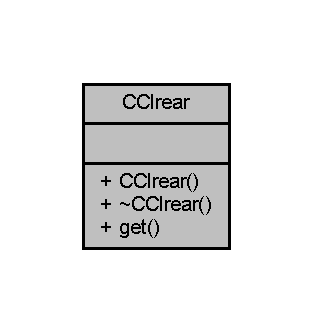
\includegraphics[width=150pt]{class_c_clrear__coll__graph}
\end{center}
\end{figure}
\subsection*{Public Member Functions}
\begin{DoxyCompactItemize}
\item 
\mbox{\Hypertarget{class_c_clrear_a66fef7166032cecdf34bfbff9caf68d4}\label{class_c_clrear_a66fef7166032cecdf34bfbff9caf68d4}} 
{\bfseries C\+Clrear} (uint32\+\_\+t size)
\item 
\mbox{\Hypertarget{class_c_clrear_ad27f3959940d997828caa2b7db457947}\label{class_c_clrear_ad27f3959940d997828caa2b7db457947}} 
const char $\ast$ {\bfseries get} () const
\end{DoxyCompactItemize}


The documentation for this class was generated from the following file\+:\begin{DoxyCompactItemize}
\item 
water\+Compute/src/C\+Water\+Open\+C\+L.\+cpp\end{DoxyCompactItemize}

\hypertarget{class_net_1_1_c_net}{}\section{Net\+:\+:C\+Net Class Reference}
\label{class_net_1_1_c_net}\index{Net\+::\+C\+Net@{Net\+::\+C\+Net}}


Server initialization class.  




{\ttfamily \#include $<$C\+Net.\+hpp$>$}



Collaboration diagram for Net\+:\+:C\+Net\+:
\nopagebreak
\begin{figure}[H]
\begin{center}
\leavevmode
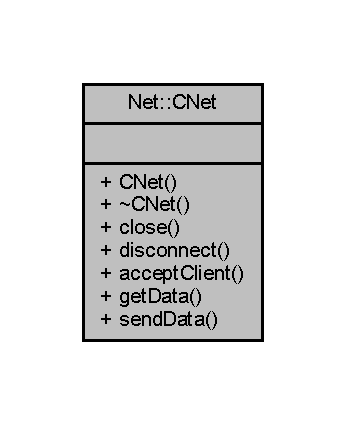
\includegraphics[width=166pt]{class_net_1_1_c_net__coll__graph}
\end{center}
\end{figure}
\subsection*{Public Member Functions}
\begin{DoxyCompactItemize}
\item 
\mbox{\hyperlink{class_net_1_1_c_net_a2e7bdcc29f062828ecac6f2caa1bbf5c}{C\+Net}} (const int max\+Con, const std\+::string \&ip, const int port)
\begin{DoxyCompactList}\small\item\em Constructor. In case of errors, he throws exceptions. \end{DoxyCompactList}\item 
\mbox{\Hypertarget{class_net_1_1_c_net_a324846d932eefbfe5316ea53f66a69dd}\label{class_net_1_1_c_net_a324846d932eefbfe5316ea53f66a69dd}} 
\mbox{\hyperlink{class_net_1_1_c_net_a324846d932eefbfe5316ea53f66a69dd}{$\sim$\+C\+Net}} ()
\begin{DoxyCompactList}\small\item\em Destructor. \end{DoxyCompactList}\item 
\mbox{\Hypertarget{class_net_1_1_c_net_a7dbe5d1a571964634d88596d7c6e7c2f}\label{class_net_1_1_c_net_a7dbe5d1a571964634d88596d7c6e7c2f}} 
void \mbox{\hyperlink{class_net_1_1_c_net_a7dbe5d1a571964634d88596d7c6e7c2f}{close}} ()
\begin{DoxyCompactList}\small\item\em Closing of clients\textquotesingle{} expectations. \end{DoxyCompactList}\item 
void \mbox{\hyperlink{class_net_1_1_c_net_a7f66009e63ed53b541331143bb2f4bfb}{disconnect}} (\mbox{\hyperlink{struct_net_1_1_s_token}{S\+Token}} \&client\+Token, Disconnect\+Reason reason)
\begin{DoxyCompactList}\small\item\em Disconnect the client. \end{DoxyCompactList}\item 
\mbox{\hyperlink{struct_net_1_1_s_token}{S\+Token}} \mbox{\hyperlink{class_net_1_1_c_net_a802a6ab154226caaa8d70423374b8034}{accept\+Client}} ()
\begin{DoxyCompactList}\small\item\em The function of connection waiting. \end{DoxyCompactList}\item 
bool \mbox{\hyperlink{class_net_1_1_c_net_a77d474d293656443de888283db8a74f0}{get\+Data}} (const \mbox{\hyperlink{struct_net_1_1_s_token}{S\+Token}} \&client\+Token, std\+::string \&data)
\begin{DoxyCompactList}\small\item\em Receiving data from the client. \end{DoxyCompactList}\item 
void \mbox{\hyperlink{class_net_1_1_c_net_a22a961e8db355efd94539336937b956b}{send\+Data}} (const \mbox{\hyperlink{struct_net_1_1_s_token}{S\+Token}} \&client\+Token, const std\+::string \&data)
\begin{DoxyCompactList}\small\item\em Sending data to the client. \end{DoxyCompactList}\end{DoxyCompactItemize}


\subsection{Detailed Description}
Server initialization class. 

\subsection{Constructor \& Destructor Documentation}
\mbox{\Hypertarget{class_net_1_1_c_net_a2e7bdcc29f062828ecac6f2caa1bbf5c}\label{class_net_1_1_c_net_a2e7bdcc29f062828ecac6f2caa1bbf5c}} 
\index{Net\+::\+C\+Net@{Net\+::\+C\+Net}!C\+Net@{C\+Net}}
\index{C\+Net@{C\+Net}!Net\+::\+C\+Net@{Net\+::\+C\+Net}}
\subsubsection{\texorpdfstring{C\+Net()}{CNet()}}
{\footnotesize\ttfamily Net\+::\+C\+Net\+::\+C\+Net (\begin{DoxyParamCaption}\item[{const int}]{max\+Con,  }\item[{const std\+::string \&}]{ip,  }\item[{const int}]{port }\end{DoxyParamCaption})}



Constructor. In case of errors, he throws exceptions. 

\begin{DoxySeeAlso}{See also}
Exception
\end{DoxySeeAlso}

\begin{DoxyParams}{Parameters}
{\em max\+Con} & Maximum number of connections. \\
\hline
{\em ip} & I\+Pv4. \\
\hline
{\em port} & Port number. \\
\hline
\end{DoxyParams}
Here is the call graph for this function\+:
\nopagebreak
\begin{figure}[H]
\begin{center}
\leavevmode
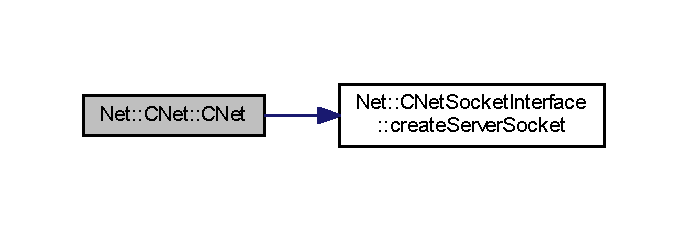
\includegraphics[width=330pt]{class_net_1_1_c_net_a2e7bdcc29f062828ecac6f2caa1bbf5c_cgraph}
\end{center}
\end{figure}


\subsection{Member Function Documentation}
\mbox{\Hypertarget{class_net_1_1_c_net_a802a6ab154226caaa8d70423374b8034}\label{class_net_1_1_c_net_a802a6ab154226caaa8d70423374b8034}} 
\index{Net\+::\+C\+Net@{Net\+::\+C\+Net}!accept\+Client@{accept\+Client}}
\index{accept\+Client@{accept\+Client}!Net\+::\+C\+Net@{Net\+::\+C\+Net}}
\subsubsection{\texorpdfstring{accept\+Client()}{acceptClient()}}
{\footnotesize\ttfamily \mbox{\hyperlink{struct_net_1_1_s_token}{Net\+::\+S\+Token}} Net\+::\+C\+Net\+::accept\+Client (\begin{DoxyParamCaption}{ }\end{DoxyParamCaption})}



The function of connection waiting. 

\begin{DoxyReturn}{Returns}
\mbox{\hyperlink{struct_net_1_1_s_token}{S\+Token}} Data about the client. If socket\+\_\+ = -\/1, then a client receive error occurred. 
\end{DoxyReturn}
Here is the call graph for this function\+:
\nopagebreak
\begin{figure}[H]
\begin{center}
\leavevmode
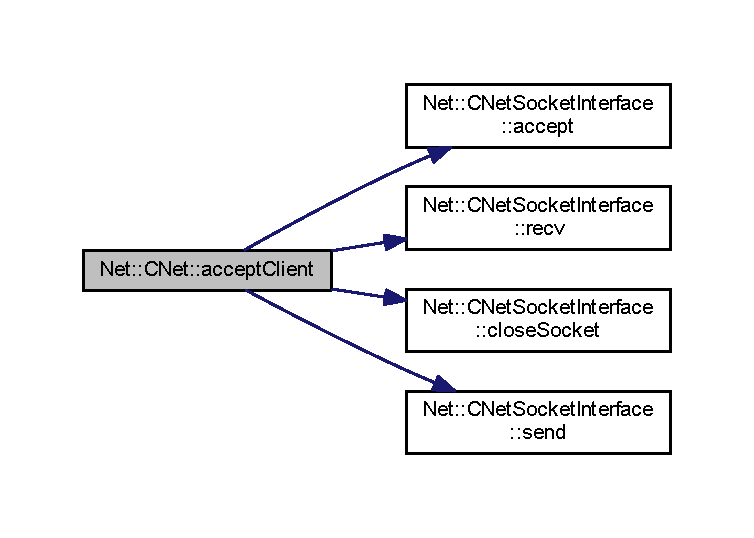
\includegraphics[width=350pt]{class_net_1_1_c_net_a802a6ab154226caaa8d70423374b8034_cgraph}
\end{center}
\end{figure}
\mbox{\Hypertarget{class_net_1_1_c_net_a7f66009e63ed53b541331143bb2f4bfb}\label{class_net_1_1_c_net_a7f66009e63ed53b541331143bb2f4bfb}} 
\index{Net\+::\+C\+Net@{Net\+::\+C\+Net}!disconnect@{disconnect}}
\index{disconnect@{disconnect}!Net\+::\+C\+Net@{Net\+::\+C\+Net}}
\subsubsection{\texorpdfstring{disconnect()}{disconnect()}}
{\footnotesize\ttfamily void Net\+::\+C\+Net\+::disconnect (\begin{DoxyParamCaption}\item[{\mbox{\hyperlink{struct_net_1_1_s_token}{S\+Token}} \&}]{client\+Token,  }\item[{Disconnect\+Reason}]{reason }\end{DoxyParamCaption})}



Disconnect the client. 


\begin{DoxyParams}{Parameters}
{\em client\+Token} & Client token. \\
\hline
{\em reason} & The cause of the connection failure. \\
\hline
\end{DoxyParams}
Here is the call graph for this function\+:
\nopagebreak
\begin{figure}[H]
\begin{center}
\leavevmode
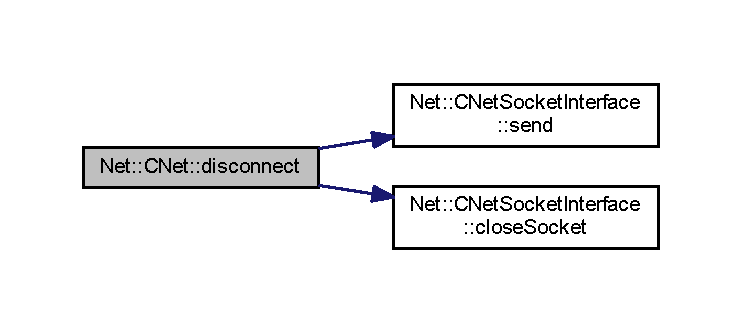
\includegraphics[width=350pt]{class_net_1_1_c_net_a7f66009e63ed53b541331143bb2f4bfb_cgraph}
\end{center}
\end{figure}
Here is the caller graph for this function\+:
\nopagebreak
\begin{figure}[H]
\begin{center}
\leavevmode
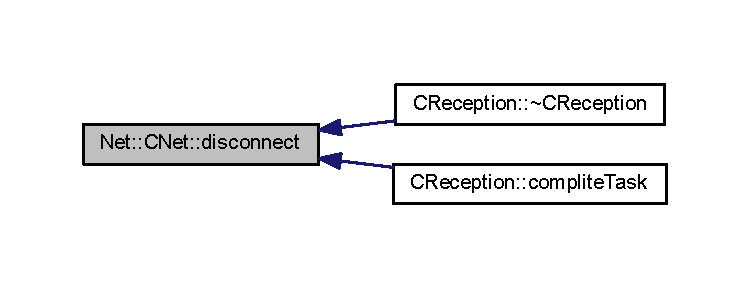
\includegraphics[width=350pt]{class_net_1_1_c_net_a7f66009e63ed53b541331143bb2f4bfb_icgraph}
\end{center}
\end{figure}
\mbox{\Hypertarget{class_net_1_1_c_net_a77d474d293656443de888283db8a74f0}\label{class_net_1_1_c_net_a77d474d293656443de888283db8a74f0}} 
\index{Net\+::\+C\+Net@{Net\+::\+C\+Net}!get\+Data@{get\+Data}}
\index{get\+Data@{get\+Data}!Net\+::\+C\+Net@{Net\+::\+C\+Net}}
\subsubsection{\texorpdfstring{get\+Data()}{getData()}}
{\footnotesize\ttfamily bool Net\+::\+C\+Net\+::get\+Data (\begin{DoxyParamCaption}\item[{const \mbox{\hyperlink{struct_net_1_1_s_token}{S\+Token}} \&}]{client\+Token,  }\item[{std\+::string \&}]{data }\end{DoxyParamCaption})}



Receiving data from the client. 


\begin{DoxyParams}{Parameters}
{\em client\+Token} & Information about the client. \\
\hline
{\em data} & Data. \\
\hline
\end{DoxyParams}
Here is the call graph for this function\+:
\nopagebreak
\begin{figure}[H]
\begin{center}
\leavevmode
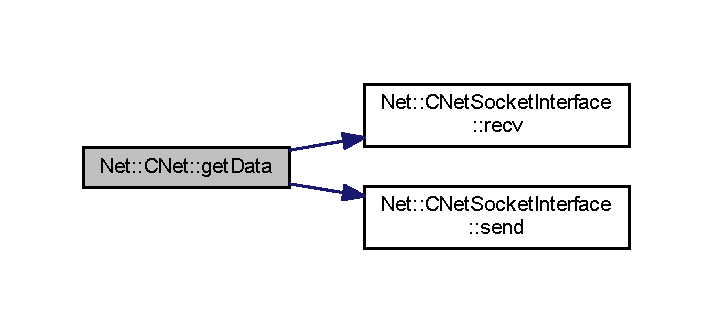
\includegraphics[width=342pt]{class_net_1_1_c_net_a77d474d293656443de888283db8a74f0_cgraph}
\end{center}
\end{figure}
\mbox{\Hypertarget{class_net_1_1_c_net_a22a961e8db355efd94539336937b956b}\label{class_net_1_1_c_net_a22a961e8db355efd94539336937b956b}} 
\index{Net\+::\+C\+Net@{Net\+::\+C\+Net}!send\+Data@{send\+Data}}
\index{send\+Data@{send\+Data}!Net\+::\+C\+Net@{Net\+::\+C\+Net}}
\subsubsection{\texorpdfstring{send\+Data()}{sendData()}}
{\footnotesize\ttfamily void Net\+::\+C\+Net\+::send\+Data (\begin{DoxyParamCaption}\item[{const \mbox{\hyperlink{struct_net_1_1_s_token}{S\+Token}} \&}]{client\+Token,  }\item[{const std\+::string \&}]{data }\end{DoxyParamCaption})}



Sending data to the client. 


\begin{DoxyParams}{Parameters}
{\em client\+Token} & Information about the client. \\
\hline
{\em data} & Data. \\
\hline
\end{DoxyParams}
Here is the call graph for this function\+:
\nopagebreak
\begin{figure}[H]
\begin{center}
\leavevmode
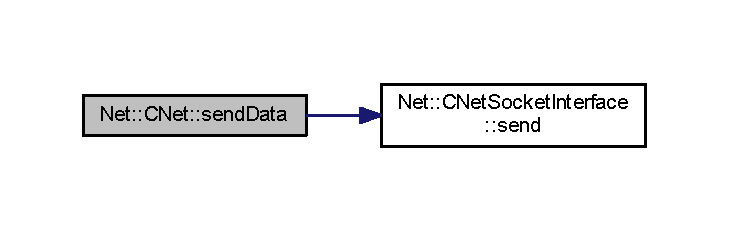
\includegraphics[width=350pt]{class_net_1_1_c_net_a22a961e8db355efd94539336937b956b_cgraph}
\end{center}
\end{figure}
Here is the caller graph for this function\+:
\nopagebreak
\begin{figure}[H]
\begin{center}
\leavevmode
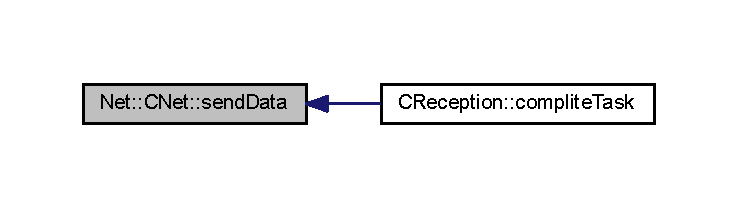
\includegraphics[width=350pt]{class_net_1_1_c_net_a22a961e8db355efd94539336937b956b_icgraph}
\end{center}
\end{figure}


The documentation for this class was generated from the following files\+:\begin{DoxyCompactItemize}
\item 
server/\+C\+Net/C\+Net.\+hpp\item 
server/\+C\+Net/C\+Net.\+cpp\end{DoxyCompactItemize}

\hypertarget{class_net_1_1_c_net_handler}{}\section{Net\+:\+:C\+Net\+Handler Class Reference}
\label{class_net_1_1_c_net_handler}\index{Net\+::\+C\+Net\+Handler@{Net\+::\+C\+Net\+Handler}}


Virtual class for creating a connection protocol handler.  




{\ttfamily \#include $<$C\+Net\+Handler.\+hpp$>$}



Inheritance diagram for Net\+:\+:C\+Net\+Handler\+:
\nopagebreak
\begin{figure}[H]
\begin{center}
\leavevmode
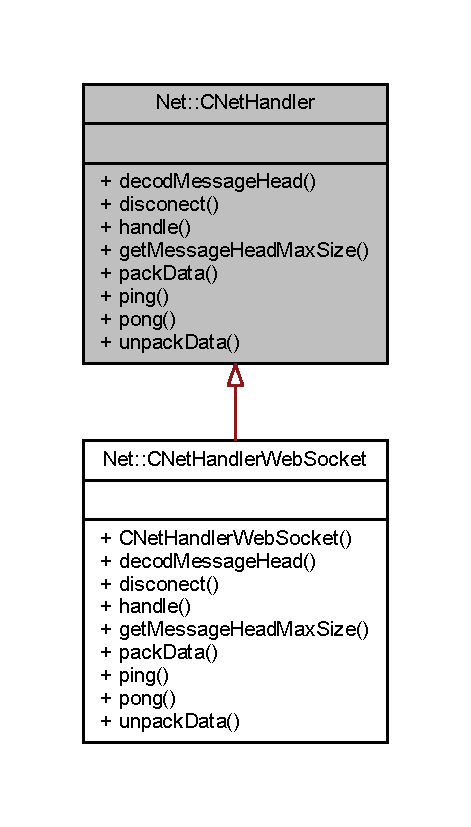
\includegraphics[width=226pt]{class_net_1_1_c_net_handler__inherit__graph}
\end{center}
\end{figure}


Collaboration diagram for Net\+:\+:C\+Net\+Handler\+:
\nopagebreak
\begin{figure}[H]
\begin{center}
\leavevmode
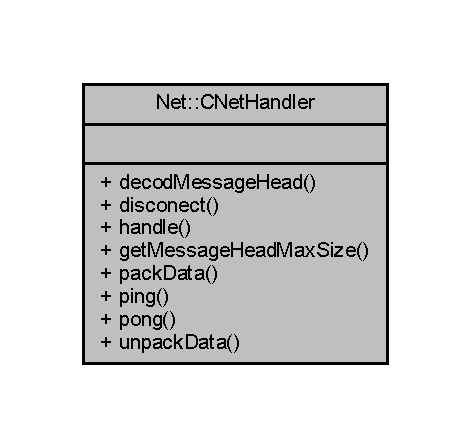
\includegraphics[width=226pt]{class_net_1_1_c_net_handler__coll__graph}
\end{center}
\end{figure}
\subsection*{Public Member Functions}
\begin{DoxyCompactItemize}
\item 
virtual \mbox{\hyperlink{struct_net_1_1_s_message_head}{S\+Message\+Head}} \mbox{\hyperlink{class_net_1_1_c_net_handler_a992b6c07fcda7c7f8ee411773b7dc3c6}{decod\+Message\+Head}} (const std\+::string \&message\+Head)=0
\begin{DoxyCompactList}\small\item\em Function for decoding the message header. \end{DoxyCompactList}\item 
virtual std\+::string \mbox{\hyperlink{class_net_1_1_c_net_handler_a1f43099b8631032d4555a326dd71f4d1}{disconect}} (Disconnect\+Reason reason)=0
\begin{DoxyCompactList}\small\item\em A function for correctly terminating a connection. \end{DoxyCompactList}\item 
virtual std\+::string \mbox{\hyperlink{class_net_1_1_c_net_handler_a7bd761afe7eff3897b840db84f870135}{handle}} (const std\+::string \&head, bool \&is\+Send\+Answer)=0
\begin{DoxyCompactList}\small\item\em Puncturing header processing function. Returns the response to the query. If the protocol header does not apply to the current handler, an empty response is returned. \end{DoxyCompactList}\item 
virtual uint \mbox{\hyperlink{class_net_1_1_c_net_handler_a6d0a79a8fc8126f6bf90e348c90152a7}{get\+Message\+Head\+Max\+Size}} ()=0
\begin{DoxyCompactList}\small\item\em Get the maximum size of the message header. \end{DoxyCompactList}\item 
virtual std\+::string \mbox{\hyperlink{class_net_1_1_c_net_handler_a9e8b6b44b05d2acb7b7cb28c57bedcb8}{pack\+Data}} (const std\+::string \&data, const bool is\+Use\+Mask)=0
\begin{DoxyCompactList}\small\item\em Packs the data in accordance with the transmission protocol. \end{DoxyCompactList}\item 
virtual std\+::string \mbox{\hyperlink{class_net_1_1_c_net_handler_af905edf8c2f5dee54f278f78d66b400d}{ping}} ()=0
\begin{DoxyCompactList}\small\item\em Receive a package to send a ping request. \end{DoxyCompactList}\item 
virtual std\+::string \mbox{\hyperlink{class_net_1_1_c_net_handler_a818189d3332d68cf28d30ec31bed0e17}{pong}} ()=0
\begin{DoxyCompactList}\small\item\em Receive a package to send a ping response. \end{DoxyCompactList}\item 
virtual std\+::string \mbox{\hyperlink{class_net_1_1_c_net_handler_aea2d09ea3bfa8d7a13ace3aec6ba9356}{unpack\+Data}} (const \mbox{\hyperlink{struct_net_1_1_s_message_head}{S\+Message\+Head}} \&head, const std\+::string \&data\+Pack)=0
\begin{DoxyCompactList}\small\item\em Unpacks the data according to the transmission protocol. \end{DoxyCompactList}\end{DoxyCompactItemize}


\subsection{Detailed Description}
Virtual class for creating a connection protocol handler. 

\subsection{Member Function Documentation}
\mbox{\Hypertarget{class_net_1_1_c_net_handler_a992b6c07fcda7c7f8ee411773b7dc3c6}\label{class_net_1_1_c_net_handler_a992b6c07fcda7c7f8ee411773b7dc3c6}} 
\index{Net\+::\+C\+Net\+Handler@{Net\+::\+C\+Net\+Handler}!decod\+Message\+Head@{decod\+Message\+Head}}
\index{decod\+Message\+Head@{decod\+Message\+Head}!Net\+::\+C\+Net\+Handler@{Net\+::\+C\+Net\+Handler}}
\subsubsection{\texorpdfstring{decod\+Message\+Head()}{decodMessageHead()}}
{\footnotesize\ttfamily virtual \mbox{\hyperlink{struct_net_1_1_s_message_head}{S\+Message\+Head}} Net\+::\+C\+Net\+Handler\+::decod\+Message\+Head (\begin{DoxyParamCaption}\item[{const std\+::string \&}]{message\+Head }\end{DoxyParamCaption})\hspace{0.3cm}{\ttfamily [pure virtual]}}



Function for decoding the message header. 


\begin{DoxyParams}{Parameters}
{\em message\+Head} & The part of the message or the entire message containing the title. \\
\hline
\end{DoxyParams}
\begin{DoxyReturn}{Returns}
\mbox{\hyperlink{struct_net_1_1_s_message_head}{S\+Message\+Head}} Decrypted message header. 
\end{DoxyReturn}


Implemented in \mbox{\hyperlink{class_net_1_1_c_net_handler_web_socket_a26a43acb16b7879df22aa3ce3fc1d172}{Net\+::\+C\+Net\+Handler\+Web\+Socket}}.

\mbox{\Hypertarget{class_net_1_1_c_net_handler_a1f43099b8631032d4555a326dd71f4d1}\label{class_net_1_1_c_net_handler_a1f43099b8631032d4555a326dd71f4d1}} 
\index{Net\+::\+C\+Net\+Handler@{Net\+::\+C\+Net\+Handler}!disconect@{disconect}}
\index{disconect@{disconect}!Net\+::\+C\+Net\+Handler@{Net\+::\+C\+Net\+Handler}}
\subsubsection{\texorpdfstring{disconect()}{disconect()}}
{\footnotesize\ttfamily virtual std\+::string Net\+::\+C\+Net\+Handler\+::disconect (\begin{DoxyParamCaption}\item[{Disconnect\+Reason}]{reason }\end{DoxyParamCaption})\hspace{0.3cm}{\ttfamily [pure virtual]}}



A function for correctly terminating a connection. 


\begin{DoxyParams}{Parameters}
{\em reason} & The cause of the connection failure. \\
\hline
\end{DoxyParams}
\begin{DoxyReturn}{Returns}
std\+::string Package to send. 
\end{DoxyReturn}


Implemented in \mbox{\hyperlink{class_net_1_1_c_net_handler_web_socket_ac5a2c812c7a1fdb426265a4590409ae3}{Net\+::\+C\+Net\+Handler\+Web\+Socket}}.

\mbox{\Hypertarget{class_net_1_1_c_net_handler_a6d0a79a8fc8126f6bf90e348c90152a7}\label{class_net_1_1_c_net_handler_a6d0a79a8fc8126f6bf90e348c90152a7}} 
\index{Net\+::\+C\+Net\+Handler@{Net\+::\+C\+Net\+Handler}!get\+Message\+Head\+Max\+Size@{get\+Message\+Head\+Max\+Size}}
\index{get\+Message\+Head\+Max\+Size@{get\+Message\+Head\+Max\+Size}!Net\+::\+C\+Net\+Handler@{Net\+::\+C\+Net\+Handler}}
\subsubsection{\texorpdfstring{get\+Message\+Head\+Max\+Size()}{getMessageHeadMaxSize()}}
{\footnotesize\ttfamily virtual uint Net\+::\+C\+Net\+Handler\+::get\+Message\+Head\+Max\+Size (\begin{DoxyParamCaption}{ }\end{DoxyParamCaption})\hspace{0.3cm}{\ttfamily [pure virtual]}}



Get the maximum size of the message header. 

\begin{DoxyReturn}{Returns}
uint Head size. 
\end{DoxyReturn}


Implemented in \mbox{\hyperlink{class_net_1_1_c_net_handler_web_socket_a5c3fa1c1f926119482b25159afffb6cd}{Net\+::\+C\+Net\+Handler\+Web\+Socket}}.

\mbox{\Hypertarget{class_net_1_1_c_net_handler_a7bd761afe7eff3897b840db84f870135}\label{class_net_1_1_c_net_handler_a7bd761afe7eff3897b840db84f870135}} 
\index{Net\+::\+C\+Net\+Handler@{Net\+::\+C\+Net\+Handler}!handle@{handle}}
\index{handle@{handle}!Net\+::\+C\+Net\+Handler@{Net\+::\+C\+Net\+Handler}}
\subsubsection{\texorpdfstring{handle()}{handle()}}
{\footnotesize\ttfamily virtual std\+::string Net\+::\+C\+Net\+Handler\+::handle (\begin{DoxyParamCaption}\item[{const std\+::string \&}]{head,  }\item[{bool \&}]{is\+Send\+Answer }\end{DoxyParamCaption})\hspace{0.3cm}{\ttfamily [pure virtual]}}



Puncturing header processing function. Returns the response to the query. If the protocol header does not apply to the current handler, an empty response is returned. 


\begin{DoxyParams}{Parameters}
{\em head} & Protocol header for connection setup. \\
\hline
{\em is\+Send\+Answer} & Sets whether the response should be sent. \\
\hline
\end{DoxyParams}
\begin{DoxyReturn}{Returns}
std\+::string Answer. 
\end{DoxyReturn}


Implemented in \mbox{\hyperlink{class_net_1_1_c_net_handler_web_socket_ad4c16a911b8cb26f69dda807b5ca2c70}{Net\+::\+C\+Net\+Handler\+Web\+Socket}}.

\mbox{\Hypertarget{class_net_1_1_c_net_handler_a9e8b6b44b05d2acb7b7cb28c57bedcb8}\label{class_net_1_1_c_net_handler_a9e8b6b44b05d2acb7b7cb28c57bedcb8}} 
\index{Net\+::\+C\+Net\+Handler@{Net\+::\+C\+Net\+Handler}!pack\+Data@{pack\+Data}}
\index{pack\+Data@{pack\+Data}!Net\+::\+C\+Net\+Handler@{Net\+::\+C\+Net\+Handler}}
\subsubsection{\texorpdfstring{pack\+Data()}{packData()}}
{\footnotesize\ttfamily virtual std\+::string Net\+::\+C\+Net\+Handler\+::pack\+Data (\begin{DoxyParamCaption}\item[{const std\+::string \&}]{data,  }\item[{const bool}]{is\+Use\+Mask }\end{DoxyParamCaption})\hspace{0.3cm}{\ttfamily [pure virtual]}}



Packs the data in accordance with the transmission protocol. 


\begin{DoxyParams}{Parameters}
{\em data} & Data for packaging. \\
\hline
{\em is\+Use\+Mask} & Use the mask when packing. \\
\hline
\end{DoxyParams}
\begin{DoxyReturn}{Returns}
std\+::string Package to send. 
\end{DoxyReturn}


Implemented in \mbox{\hyperlink{class_net_1_1_c_net_handler_web_socket_aa408c8c686da45c36969a7dcf7478daa}{Net\+::\+C\+Net\+Handler\+Web\+Socket}}.

\mbox{\Hypertarget{class_net_1_1_c_net_handler_af905edf8c2f5dee54f278f78d66b400d}\label{class_net_1_1_c_net_handler_af905edf8c2f5dee54f278f78d66b400d}} 
\index{Net\+::\+C\+Net\+Handler@{Net\+::\+C\+Net\+Handler}!ping@{ping}}
\index{ping@{ping}!Net\+::\+C\+Net\+Handler@{Net\+::\+C\+Net\+Handler}}
\subsubsection{\texorpdfstring{ping()}{ping()}}
{\footnotesize\ttfamily virtual std\+::string Net\+::\+C\+Net\+Handler\+::ping (\begin{DoxyParamCaption}{ }\end{DoxyParamCaption})\hspace{0.3cm}{\ttfamily [pure virtual]}}



Receive a package to send a ping request. 

\begin{DoxyReturn}{Returns}
std\+::string Package to send. 
\end{DoxyReturn}


Implemented in \mbox{\hyperlink{class_net_1_1_c_net_handler_web_socket_aa19e13e42fa3a31ab8d8a8291af4b5e6}{Net\+::\+C\+Net\+Handler\+Web\+Socket}}.

\mbox{\Hypertarget{class_net_1_1_c_net_handler_a818189d3332d68cf28d30ec31bed0e17}\label{class_net_1_1_c_net_handler_a818189d3332d68cf28d30ec31bed0e17}} 
\index{Net\+::\+C\+Net\+Handler@{Net\+::\+C\+Net\+Handler}!pong@{pong}}
\index{pong@{pong}!Net\+::\+C\+Net\+Handler@{Net\+::\+C\+Net\+Handler}}
\subsubsection{\texorpdfstring{pong()}{pong()}}
{\footnotesize\ttfamily virtual std\+::string Net\+::\+C\+Net\+Handler\+::pong (\begin{DoxyParamCaption}{ }\end{DoxyParamCaption})\hspace{0.3cm}{\ttfamily [pure virtual]}}



Receive a package to send a ping response. 

\begin{DoxyReturn}{Returns}
std\+::string Package to send. 
\end{DoxyReturn}


Implemented in \mbox{\hyperlink{class_net_1_1_c_net_handler_web_socket_a51d3618ba601abc5047cf0da91b8a374}{Net\+::\+C\+Net\+Handler\+Web\+Socket}}.

\mbox{\Hypertarget{class_net_1_1_c_net_handler_aea2d09ea3bfa8d7a13ace3aec6ba9356}\label{class_net_1_1_c_net_handler_aea2d09ea3bfa8d7a13ace3aec6ba9356}} 
\index{Net\+::\+C\+Net\+Handler@{Net\+::\+C\+Net\+Handler}!unpack\+Data@{unpack\+Data}}
\index{unpack\+Data@{unpack\+Data}!Net\+::\+C\+Net\+Handler@{Net\+::\+C\+Net\+Handler}}
\subsubsection{\texorpdfstring{unpack\+Data()}{unpackData()}}
{\footnotesize\ttfamily virtual std\+::string Net\+::\+C\+Net\+Handler\+::unpack\+Data (\begin{DoxyParamCaption}\item[{const \mbox{\hyperlink{struct_net_1_1_s_message_head}{S\+Message\+Head}} \&}]{head,  }\item[{const std\+::string \&}]{data\+Pack }\end{DoxyParamCaption})\hspace{0.3cm}{\ttfamily [pure virtual]}}



Unpacks the data according to the transmission protocol. 


\begin{DoxyParams}{Parameters}
{\em head} & Decoded message header. \\
\hline
{\em data\+Pack} & A message with the heading at the beginning. \\
\hline
\end{DoxyParams}
\begin{DoxyReturn}{Returns}
std\+::string Unpacked data. 
\end{DoxyReturn}


Implemented in \mbox{\hyperlink{class_net_1_1_c_net_handler_web_socket_a09297039609dca2d8e2c376626ef78f1}{Net\+::\+C\+Net\+Handler\+Web\+Socket}}.



The documentation for this class was generated from the following file\+:\begin{DoxyCompactItemize}
\item 
server/\+C\+Net/\+Handler/C\+Net\+Handler.\+hpp\end{DoxyCompactItemize}

\hypertarget{class_net_1_1_c_net_handler_web_socket}{}\section{Net\+:\+:C\+Net\+Handler\+Web\+Socket Class Reference}
\label{class_net_1_1_c_net_handler_web_socket}\index{Net\+::\+C\+Net\+Handler\+Web\+Socket@{Net\+::\+C\+Net\+Handler\+Web\+Socket}}


The protocol handler of the Web\+Socket.  




{\ttfamily \#include $<$C\+Net\+Handler\+Web\+Socket.\+hpp$>$}



Inheritance diagram for Net\+:\+:C\+Net\+Handler\+Web\+Socket\+:
\nopagebreak
\begin{figure}[H]
\begin{center}
\leavevmode
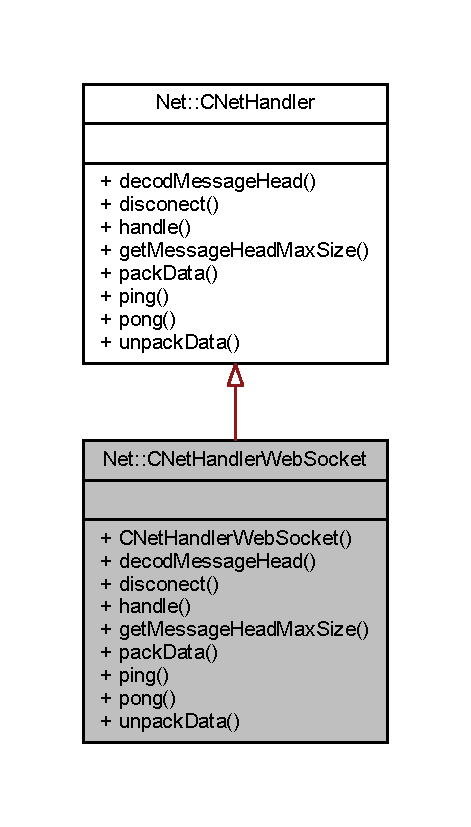
\includegraphics[width=226pt]{class_net_1_1_c_net_handler_web_socket__inherit__graph}
\end{center}
\end{figure}


Collaboration diagram for Net\+:\+:C\+Net\+Handler\+Web\+Socket\+:
\nopagebreak
\begin{figure}[H]
\begin{center}
\leavevmode
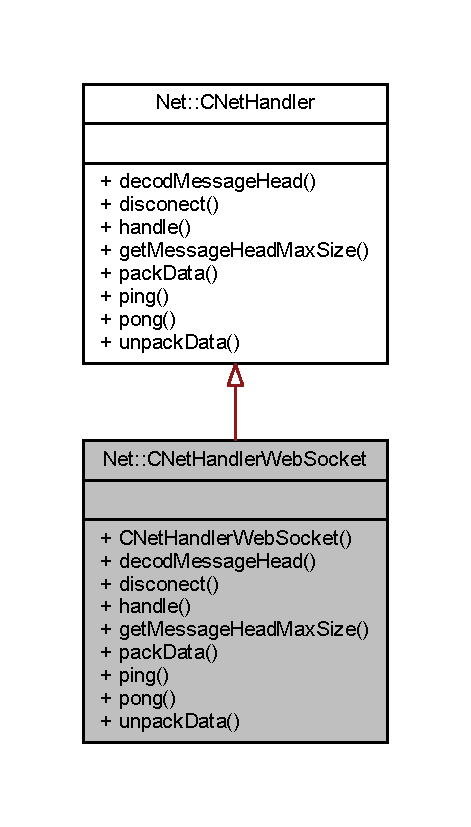
\includegraphics[width=226pt]{class_net_1_1_c_net_handler_web_socket__coll__graph}
\end{center}
\end{figure}
\subsection*{Public Member Functions}
\begin{DoxyCompactItemize}
\item 
virtual \mbox{\hyperlink{struct_net_1_1_s_message_head}{S\+Message\+Head}} \mbox{\hyperlink{class_net_1_1_c_net_handler_web_socket_a26a43acb16b7879df22aa3ce3fc1d172}{decod\+Message\+Head}} (const std\+::string \&message\+Head)
\item 
virtual std\+::string \mbox{\hyperlink{class_net_1_1_c_net_handler_web_socket_ac5a2c812c7a1fdb426265a4590409ae3}{disconect}} (Disconnect\+Reason reason)
\item 
virtual std\+::string \mbox{\hyperlink{class_net_1_1_c_net_handler_web_socket_ad4c16a911b8cb26f69dda807b5ca2c70}{handle}} (const std\+::string \&head, bool \&is\+Send\+Answer)
\item 
virtual uint \mbox{\hyperlink{class_net_1_1_c_net_handler_web_socket_a5c3fa1c1f926119482b25159afffb6cd}{get\+Message\+Head\+Max\+Size}} ()
\item 
virtual std\+::string \mbox{\hyperlink{class_net_1_1_c_net_handler_web_socket_aa408c8c686da45c36969a7dcf7478daa}{pack\+Data}} (const std\+::string \&data, const bool is\+Use\+Mask)
\item 
virtual std\+::string \mbox{\hyperlink{class_net_1_1_c_net_handler_web_socket_aa19e13e42fa3a31ab8d8a8291af4b5e6}{ping}} ()
\item 
virtual std\+::string \mbox{\hyperlink{class_net_1_1_c_net_handler_web_socket_a51d3618ba601abc5047cf0da91b8a374}{pong}} ()
\item 
virtual std\+::string \mbox{\hyperlink{class_net_1_1_c_net_handler_web_socket_a09297039609dca2d8e2c376626ef78f1}{unpack\+Data}} (const \mbox{\hyperlink{struct_net_1_1_s_message_head}{S\+Message\+Head}} \&head, const std\+::string \&data\+Pack)
\end{DoxyCompactItemize}


\subsection{Detailed Description}
The protocol handler of the Web\+Socket. 

\subsection{Member Function Documentation}
\mbox{\Hypertarget{class_net_1_1_c_net_handler_web_socket_a26a43acb16b7879df22aa3ce3fc1d172}\label{class_net_1_1_c_net_handler_web_socket_a26a43acb16b7879df22aa3ce3fc1d172}} 
\index{Net\+::\+C\+Net\+Handler\+Web\+Socket@{Net\+::\+C\+Net\+Handler\+Web\+Socket}!decod\+Message\+Head@{decod\+Message\+Head}}
\index{decod\+Message\+Head@{decod\+Message\+Head}!Net\+::\+C\+Net\+Handler\+Web\+Socket@{Net\+::\+C\+Net\+Handler\+Web\+Socket}}
\subsubsection{\texorpdfstring{decod\+Message\+Head()}{decodMessageHead()}}
{\footnotesize\ttfamily \mbox{\hyperlink{struct_net_1_1_s_message_head}{S\+Message\+Head}} C\+Net\+Handler\+Web\+Socket\+::decod\+Message\+Head (\begin{DoxyParamCaption}\item[{const std\+::string \&}]{message\+Head }\end{DoxyParamCaption})\hspace{0.3cm}{\ttfamily [virtual]}}

\begin{DoxySeeAlso}{See also}
\mbox{\hyperlink{class_net_1_1_c_net_handler_a992b6c07fcda7c7f8ee411773b7dc3c6}{Net\+::\+C\+Net\+Handler\+::decod\+Message\+Head}} 
\end{DoxySeeAlso}


Implements \mbox{\hyperlink{class_net_1_1_c_net_handler_a992b6c07fcda7c7f8ee411773b7dc3c6}{Net\+::\+C\+Net\+Handler}}.

\mbox{\Hypertarget{class_net_1_1_c_net_handler_web_socket_ac5a2c812c7a1fdb426265a4590409ae3}\label{class_net_1_1_c_net_handler_web_socket_ac5a2c812c7a1fdb426265a4590409ae3}} 
\index{Net\+::\+C\+Net\+Handler\+Web\+Socket@{Net\+::\+C\+Net\+Handler\+Web\+Socket}!disconect@{disconect}}
\index{disconect@{disconect}!Net\+::\+C\+Net\+Handler\+Web\+Socket@{Net\+::\+C\+Net\+Handler\+Web\+Socket}}
\subsubsection{\texorpdfstring{disconect()}{disconect()}}
{\footnotesize\ttfamily std\+::string C\+Net\+Handler\+Web\+Socket\+::disconect (\begin{DoxyParamCaption}\item[{Disconnect\+Reason}]{reason }\end{DoxyParamCaption})\hspace{0.3cm}{\ttfamily [virtual]}}

\begin{DoxySeeAlso}{See also}
\mbox{\hyperlink{class_net_1_1_c_net_handler_a1f43099b8631032d4555a326dd71f4d1}{Net\+::\+C\+Net\+Handler\+::disconect}} 
\end{DoxySeeAlso}


Implements \mbox{\hyperlink{class_net_1_1_c_net_handler_a1f43099b8631032d4555a326dd71f4d1}{Net\+::\+C\+Net\+Handler}}.

\mbox{\Hypertarget{class_net_1_1_c_net_handler_web_socket_a5c3fa1c1f926119482b25159afffb6cd}\label{class_net_1_1_c_net_handler_web_socket_a5c3fa1c1f926119482b25159afffb6cd}} 
\index{Net\+::\+C\+Net\+Handler\+Web\+Socket@{Net\+::\+C\+Net\+Handler\+Web\+Socket}!get\+Message\+Head\+Max\+Size@{get\+Message\+Head\+Max\+Size}}
\index{get\+Message\+Head\+Max\+Size@{get\+Message\+Head\+Max\+Size}!Net\+::\+C\+Net\+Handler\+Web\+Socket@{Net\+::\+C\+Net\+Handler\+Web\+Socket}}
\subsubsection{\texorpdfstring{get\+Message\+Head\+Max\+Size()}{getMessageHeadMaxSize()}}
{\footnotesize\ttfamily uint C\+Net\+Handler\+Web\+Socket\+::get\+Message\+Head\+Max\+Size (\begin{DoxyParamCaption}{ }\end{DoxyParamCaption})\hspace{0.3cm}{\ttfamily [virtual]}}

\begin{DoxySeeAlso}{See also}
\mbox{\hyperlink{class_net_1_1_c_net_handler_a6d0a79a8fc8126f6bf90e348c90152a7}{Net\+::\+C\+Net\+Handler\+::get\+Message\+Head\+Max\+Size}} 
\end{DoxySeeAlso}


Implements \mbox{\hyperlink{class_net_1_1_c_net_handler_a6d0a79a8fc8126f6bf90e348c90152a7}{Net\+::\+C\+Net\+Handler}}.

\mbox{\Hypertarget{class_net_1_1_c_net_handler_web_socket_ad4c16a911b8cb26f69dda807b5ca2c70}\label{class_net_1_1_c_net_handler_web_socket_ad4c16a911b8cb26f69dda807b5ca2c70}} 
\index{Net\+::\+C\+Net\+Handler\+Web\+Socket@{Net\+::\+C\+Net\+Handler\+Web\+Socket}!handle@{handle}}
\index{handle@{handle}!Net\+::\+C\+Net\+Handler\+Web\+Socket@{Net\+::\+C\+Net\+Handler\+Web\+Socket}}
\subsubsection{\texorpdfstring{handle()}{handle()}}
{\footnotesize\ttfamily std\+::string C\+Net\+Handler\+Web\+Socket\+::handle (\begin{DoxyParamCaption}\item[{const std\+::string \&}]{head,  }\item[{bool \&}]{is\+Send\+Answer }\end{DoxyParamCaption})\hspace{0.3cm}{\ttfamily [virtual]}}

\begin{DoxySeeAlso}{See also}
\mbox{\hyperlink{class_net_1_1_c_net_handler_a7bd761afe7eff3897b840db84f870135}{Net\+::\+C\+Net\+Handler\+::handle}} 
\end{DoxySeeAlso}


Implements \mbox{\hyperlink{class_net_1_1_c_net_handler_a7bd761afe7eff3897b840db84f870135}{Net\+::\+C\+Net\+Handler}}.

\mbox{\Hypertarget{class_net_1_1_c_net_handler_web_socket_aa408c8c686da45c36969a7dcf7478daa}\label{class_net_1_1_c_net_handler_web_socket_aa408c8c686da45c36969a7dcf7478daa}} 
\index{Net\+::\+C\+Net\+Handler\+Web\+Socket@{Net\+::\+C\+Net\+Handler\+Web\+Socket}!pack\+Data@{pack\+Data}}
\index{pack\+Data@{pack\+Data}!Net\+::\+C\+Net\+Handler\+Web\+Socket@{Net\+::\+C\+Net\+Handler\+Web\+Socket}}
\subsubsection{\texorpdfstring{pack\+Data()}{packData()}}
{\footnotesize\ttfamily std\+::string C\+Net\+Handler\+Web\+Socket\+::pack\+Data (\begin{DoxyParamCaption}\item[{const std\+::string \&}]{data,  }\item[{const bool}]{is\+Use\+Mask }\end{DoxyParamCaption})\hspace{0.3cm}{\ttfamily [virtual]}}

\begin{DoxySeeAlso}{See also}
\mbox{\hyperlink{class_net_1_1_c_net_handler_a9e8b6b44b05d2acb7b7cb28c57bedcb8}{Net\+::\+C\+Net\+Handler\+::pack\+Data}} 
\end{DoxySeeAlso}


Implements \mbox{\hyperlink{class_net_1_1_c_net_handler_a9e8b6b44b05d2acb7b7cb28c57bedcb8}{Net\+::\+C\+Net\+Handler}}.

\mbox{\Hypertarget{class_net_1_1_c_net_handler_web_socket_aa19e13e42fa3a31ab8d8a8291af4b5e6}\label{class_net_1_1_c_net_handler_web_socket_aa19e13e42fa3a31ab8d8a8291af4b5e6}} 
\index{Net\+::\+C\+Net\+Handler\+Web\+Socket@{Net\+::\+C\+Net\+Handler\+Web\+Socket}!ping@{ping}}
\index{ping@{ping}!Net\+::\+C\+Net\+Handler\+Web\+Socket@{Net\+::\+C\+Net\+Handler\+Web\+Socket}}
\subsubsection{\texorpdfstring{ping()}{ping()}}
{\footnotesize\ttfamily std\+::string C\+Net\+Handler\+Web\+Socket\+::ping (\begin{DoxyParamCaption}{ }\end{DoxyParamCaption})\hspace{0.3cm}{\ttfamily [virtual]}}

\begin{DoxySeeAlso}{See also}
\mbox{\hyperlink{class_net_1_1_c_net_handler_af905edf8c2f5dee54f278f78d66b400d}{Net\+::\+C\+Net\+Handler\+::ping}} 
\end{DoxySeeAlso}


Implements \mbox{\hyperlink{class_net_1_1_c_net_handler_af905edf8c2f5dee54f278f78d66b400d}{Net\+::\+C\+Net\+Handler}}.

\mbox{\Hypertarget{class_net_1_1_c_net_handler_web_socket_a51d3618ba601abc5047cf0da91b8a374}\label{class_net_1_1_c_net_handler_web_socket_a51d3618ba601abc5047cf0da91b8a374}} 
\index{Net\+::\+C\+Net\+Handler\+Web\+Socket@{Net\+::\+C\+Net\+Handler\+Web\+Socket}!pong@{pong}}
\index{pong@{pong}!Net\+::\+C\+Net\+Handler\+Web\+Socket@{Net\+::\+C\+Net\+Handler\+Web\+Socket}}
\subsubsection{\texorpdfstring{pong()}{pong()}}
{\footnotesize\ttfamily std\+::string C\+Net\+Handler\+Web\+Socket\+::pong (\begin{DoxyParamCaption}{ }\end{DoxyParamCaption})\hspace{0.3cm}{\ttfamily [virtual]}}

\begin{DoxySeeAlso}{See also}
\mbox{\hyperlink{class_net_1_1_c_net_handler_a818189d3332d68cf28d30ec31bed0e17}{Net\+::\+C\+Net\+Handler\+::pong}} 
\end{DoxySeeAlso}


Implements \mbox{\hyperlink{class_net_1_1_c_net_handler_a818189d3332d68cf28d30ec31bed0e17}{Net\+::\+C\+Net\+Handler}}.

\mbox{\Hypertarget{class_net_1_1_c_net_handler_web_socket_a09297039609dca2d8e2c376626ef78f1}\label{class_net_1_1_c_net_handler_web_socket_a09297039609dca2d8e2c376626ef78f1}} 
\index{Net\+::\+C\+Net\+Handler\+Web\+Socket@{Net\+::\+C\+Net\+Handler\+Web\+Socket}!unpack\+Data@{unpack\+Data}}
\index{unpack\+Data@{unpack\+Data}!Net\+::\+C\+Net\+Handler\+Web\+Socket@{Net\+::\+C\+Net\+Handler\+Web\+Socket}}
\subsubsection{\texorpdfstring{unpack\+Data()}{unpackData()}}
{\footnotesize\ttfamily std\+::string C\+Net\+Handler\+Web\+Socket\+::unpack\+Data (\begin{DoxyParamCaption}\item[{const \mbox{\hyperlink{struct_net_1_1_s_message_head}{S\+Message\+Head}} \&}]{head,  }\item[{const std\+::string \&}]{data\+Pack }\end{DoxyParamCaption})\hspace{0.3cm}{\ttfamily [virtual]}}

\begin{DoxySeeAlso}{See also}
\mbox{\hyperlink{class_net_1_1_c_net_handler_aea2d09ea3bfa8d7a13ace3aec6ba9356}{Net\+::\+C\+Net\+Handler\+::unpack\+Data}} 
\end{DoxySeeAlso}


Implements \mbox{\hyperlink{class_net_1_1_c_net_handler_aea2d09ea3bfa8d7a13ace3aec6ba9356}{Net\+::\+C\+Net\+Handler}}.



The documentation for this class was generated from the following files\+:\begin{DoxyCompactItemize}
\item 
server/\+C\+Net/\+Handler/C\+Net\+Handler\+Web\+Socket.\+hpp\item 
server/\+C\+Net/\+Handler/C\+Net\+Handler\+Web\+Socket.\+cpp\end{DoxyCompactItemize}

\hypertarget{class_net_1_1_c_net_socket_interface}{}\section{Net\+:\+:C\+Net\+Socket\+Interface Class Reference}
\label{class_net_1_1_c_net_socket_interface}\index{Net\+::\+C\+Net\+Socket\+Interface@{Net\+::\+C\+Net\+Socket\+Interface}}


The interface for accessing sockets. At the beginning of using the functions, you need to initialize.  




{\ttfamily \#include $<$C\+Net\+Socket\+Interface.\+hpp$>$}



Collaboration diagram for Net\+:\+:C\+Net\+Socket\+Interface\+:
\nopagebreak
\begin{figure}[H]
\begin{center}
\leavevmode
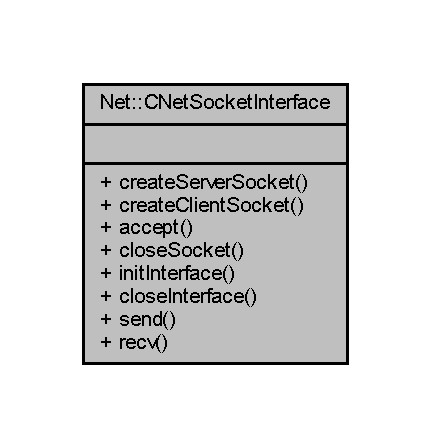
\includegraphics[width=207pt]{class_net_1_1_c_net_socket_interface__coll__graph}
\end{center}
\end{figure}
\subsection*{Static Public Member Functions}
\begin{DoxyCompactItemize}
\item 
static int \mbox{\hyperlink{class_net_1_1_c_net_socket_interface_a250ab776d6ce77b1a905904dce7bf21f}{create\+Server\+Socket}} (const uint max\+Con, const int port, const char $\ast$ip\+Adress)
\begin{DoxyCompactList}\small\item\em Create a server socket. \end{DoxyCompactList}\item 
static int \mbox{\hyperlink{class_net_1_1_c_net_socket_interface_a52ca61f347f9f08cf0ad85e45f081906}{create\+Client\+Socket}} (const int port, const char $\ast$ip\+Adress)
\begin{DoxyCompactList}\small\item\em Create a client socket. \end{DoxyCompactList}\item 
static int \mbox{\hyperlink{class_net_1_1_c_net_socket_interface_a4fceb3945002b0aa62dbc7af4afac76d}{accept}} (const int socket)
\begin{DoxyCompactList}\small\item\em Waiting for the client. \end{DoxyCompactList}\item 
static void \mbox{\hyperlink{class_net_1_1_c_net_socket_interface_a32974d8d814e78f05208eec685376df5}{close\+Socket}} (const int socket)
\begin{DoxyCompactList}\small\item\em Close socket. \end{DoxyCompactList}\item 
\mbox{\Hypertarget{class_net_1_1_c_net_socket_interface_a3f0603a3708ca966b9f37d9202761aa8}\label{class_net_1_1_c_net_socket_interface_a3f0603a3708ca966b9f37d9202761aa8}} 
static void \mbox{\hyperlink{class_net_1_1_c_net_socket_interface_a3f0603a3708ca966b9f37d9202761aa8}{init\+Interface}} ()
\begin{DoxyCompactList}\small\item\em Interface initialization function. \end{DoxyCompactList}\item 
\mbox{\Hypertarget{class_net_1_1_c_net_socket_interface_a8d07a643a30977a250d611653d05e7d2}\label{class_net_1_1_c_net_socket_interface_a8d07a643a30977a250d611653d05e7d2}} 
static void \mbox{\hyperlink{class_net_1_1_c_net_socket_interface_a8d07a643a30977a250d611653d05e7d2}{close\+Interface}} ()
\begin{DoxyCompactList}\small\item\em Function of disabling the initialized interface. \end{DoxyCompactList}\item 
static int \mbox{\hyperlink{class_net_1_1_c_net_socket_interface_ad6a594a3ebe2fd855399aabfcbe0f95e}{send}} (const int socket, const char $\ast$data, const int data\+Size)
\begin{DoxyCompactList}\small\item\em Sending data. \end{DoxyCompactList}\item 
static int \mbox{\hyperlink{class_net_1_1_c_net_socket_interface_a66531da7c243f12948bd79293d6299e2}{recv}} (const int socket, char $\ast$buffer, const int buffer\+Size)
\begin{DoxyCompactList}\small\item\em Receiving data. \end{DoxyCompactList}\end{DoxyCompactItemize}


\subsection{Detailed Description}
The interface for accessing sockets. At the beginning of using the functions, you need to initialize. 

\begin{DoxySeeAlso}{See also}
\mbox{\hyperlink{class_net_1_1_c_net_socket_interface_a3f0603a3708ca966b9f37d9202761aa8}{C\+Net\+Socket\+Interface\+::init\+Interface}} At the end of work, call \mbox{\hyperlink{class_net_1_1_c_net_socket_interface_a8d07a643a30977a250d611653d05e7d2}{close\+Interface}}. 
\end{DoxySeeAlso}


\subsection{Member Function Documentation}
\mbox{\Hypertarget{class_net_1_1_c_net_socket_interface_a4fceb3945002b0aa62dbc7af4afac76d}\label{class_net_1_1_c_net_socket_interface_a4fceb3945002b0aa62dbc7af4afac76d}} 
\index{Net\+::\+C\+Net\+Socket\+Interface@{Net\+::\+C\+Net\+Socket\+Interface}!accept@{accept}}
\index{accept@{accept}!Net\+::\+C\+Net\+Socket\+Interface@{Net\+::\+C\+Net\+Socket\+Interface}}
\subsubsection{\texorpdfstring{accept()}{accept()}}
{\footnotesize\ttfamily int Net\+::\+C\+Net\+Socket\+Interface\+::accept (\begin{DoxyParamCaption}\item[{const int}]{socket }\end{DoxyParamCaption})\hspace{0.3cm}{\ttfamily [static]}}



Waiting for the client. 


\begin{DoxyParams}{Parameters}
{\em socket} & Listen socket. \\
\hline
\end{DoxyParams}
\begin{DoxyReturn}{Returns}
int Client socket. 
\end{DoxyReturn}
Here is the caller graph for this function\+:
\nopagebreak
\begin{figure}[H]
\begin{center}
\leavevmode
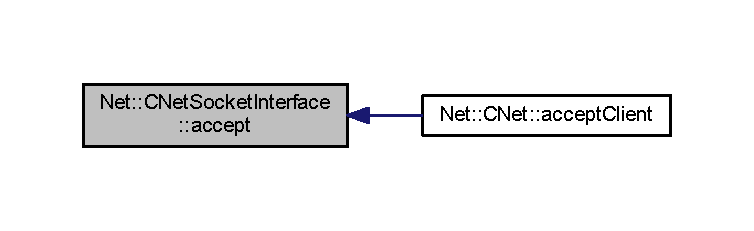
\includegraphics[width=350pt]{class_net_1_1_c_net_socket_interface_a4fceb3945002b0aa62dbc7af4afac76d_icgraph}
\end{center}
\end{figure}
\mbox{\Hypertarget{class_net_1_1_c_net_socket_interface_a32974d8d814e78f05208eec685376df5}\label{class_net_1_1_c_net_socket_interface_a32974d8d814e78f05208eec685376df5}} 
\index{Net\+::\+C\+Net\+Socket\+Interface@{Net\+::\+C\+Net\+Socket\+Interface}!close\+Socket@{close\+Socket}}
\index{close\+Socket@{close\+Socket}!Net\+::\+C\+Net\+Socket\+Interface@{Net\+::\+C\+Net\+Socket\+Interface}}
\subsubsection{\texorpdfstring{close\+Socket()}{closeSocket()}}
{\footnotesize\ttfamily void Net\+::\+C\+Net\+Socket\+Interface\+::close\+Socket (\begin{DoxyParamCaption}\item[{const int}]{socket }\end{DoxyParamCaption})\hspace{0.3cm}{\ttfamily [static]}}



Close socket. 


\begin{DoxyParams}{Parameters}
{\em socket} & Socket. \\
\hline
\end{DoxyParams}
Here is the caller graph for this function\+:
\nopagebreak
\begin{figure}[H]
\begin{center}
\leavevmode
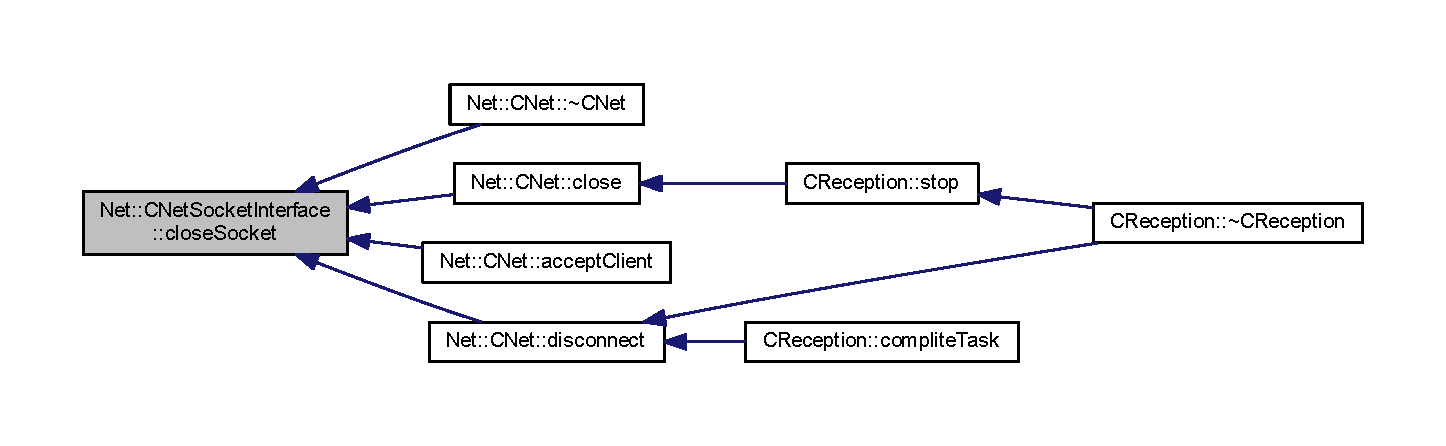
\includegraphics[width=350pt]{class_net_1_1_c_net_socket_interface_a32974d8d814e78f05208eec685376df5_icgraph}
\end{center}
\end{figure}
\mbox{\Hypertarget{class_net_1_1_c_net_socket_interface_a52ca61f347f9f08cf0ad85e45f081906}\label{class_net_1_1_c_net_socket_interface_a52ca61f347f9f08cf0ad85e45f081906}} 
\index{Net\+::\+C\+Net\+Socket\+Interface@{Net\+::\+C\+Net\+Socket\+Interface}!create\+Client\+Socket@{create\+Client\+Socket}}
\index{create\+Client\+Socket@{create\+Client\+Socket}!Net\+::\+C\+Net\+Socket\+Interface@{Net\+::\+C\+Net\+Socket\+Interface}}
\subsubsection{\texorpdfstring{create\+Client\+Socket()}{createClientSocket()}}
{\footnotesize\ttfamily int Net\+::\+C\+Net\+Socket\+Interface\+::create\+Client\+Socket (\begin{DoxyParamCaption}\item[{const int}]{port,  }\item[{const char $\ast$}]{ip\+Adress }\end{DoxyParamCaption})\hspace{0.3cm}{\ttfamily [static]}}



Create a client socket. 


\begin{DoxyParams}{Parameters}
{\em port} & \\
\hline
{\em ip\+Adress} & I\+P\+V4 \\
\hline
\end{DoxyParams}
\begin{DoxyReturn}{Returns}
int Socket. 
\end{DoxyReturn}
Here is the caller graph for this function\+:
\nopagebreak
\begin{figure}[H]
\begin{center}
\leavevmode
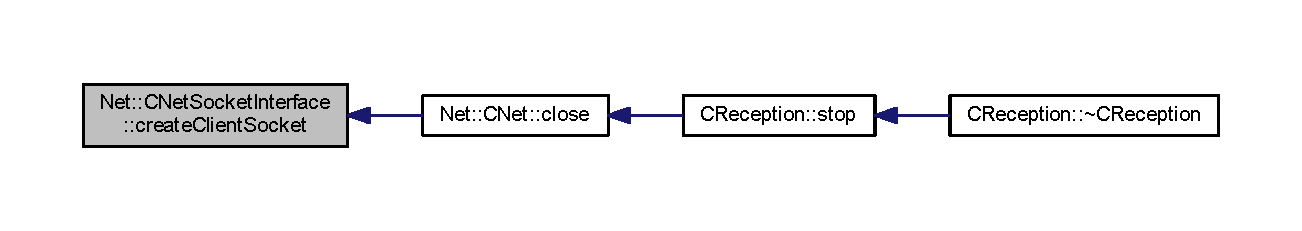
\includegraphics[width=350pt]{class_net_1_1_c_net_socket_interface_a52ca61f347f9f08cf0ad85e45f081906_icgraph}
\end{center}
\end{figure}
\mbox{\Hypertarget{class_net_1_1_c_net_socket_interface_a250ab776d6ce77b1a905904dce7bf21f}\label{class_net_1_1_c_net_socket_interface_a250ab776d6ce77b1a905904dce7bf21f}} 
\index{Net\+::\+C\+Net\+Socket\+Interface@{Net\+::\+C\+Net\+Socket\+Interface}!create\+Server\+Socket@{create\+Server\+Socket}}
\index{create\+Server\+Socket@{create\+Server\+Socket}!Net\+::\+C\+Net\+Socket\+Interface@{Net\+::\+C\+Net\+Socket\+Interface}}
\subsubsection{\texorpdfstring{create\+Server\+Socket()}{createServerSocket()}}
{\footnotesize\ttfamily int Net\+::\+C\+Net\+Socket\+Interface\+::create\+Server\+Socket (\begin{DoxyParamCaption}\item[{const uint}]{max\+Con,  }\item[{const int}]{port,  }\item[{const char $\ast$}]{ip\+Adress }\end{DoxyParamCaption})\hspace{0.3cm}{\ttfamily [static]}}



Create a server socket. 


\begin{DoxyParams}{Parameters}
{\em max\+Con} & The maximum number of connections. \\
\hline
{\em port} & \\
\hline
{\em ip\+Adress} & I\+P\+V4 \\
\hline
\end{DoxyParams}
\begin{DoxyReturn}{Returns}
int Listen socket. 
\end{DoxyReturn}
Here is the caller graph for this function\+:
\nopagebreak
\begin{figure}[H]
\begin{center}
\leavevmode
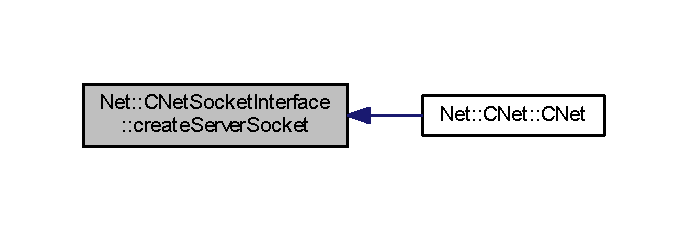
\includegraphics[width=330pt]{class_net_1_1_c_net_socket_interface_a250ab776d6ce77b1a905904dce7bf21f_icgraph}
\end{center}
\end{figure}
\mbox{\Hypertarget{class_net_1_1_c_net_socket_interface_a66531da7c243f12948bd79293d6299e2}\label{class_net_1_1_c_net_socket_interface_a66531da7c243f12948bd79293d6299e2}} 
\index{Net\+::\+C\+Net\+Socket\+Interface@{Net\+::\+C\+Net\+Socket\+Interface}!recv@{recv}}
\index{recv@{recv}!Net\+::\+C\+Net\+Socket\+Interface@{Net\+::\+C\+Net\+Socket\+Interface}}
\subsubsection{\texorpdfstring{recv()}{recv()}}
{\footnotesize\ttfamily int Net\+::\+C\+Net\+Socket\+Interface\+::recv (\begin{DoxyParamCaption}\item[{const int}]{socket,  }\item[{char $\ast$}]{buffer,  }\item[{const int}]{buffer\+Size }\end{DoxyParamCaption})\hspace{0.3cm}{\ttfamily [static]}}



Receiving data. 


\begin{DoxyParams}{Parameters}
{\em socket} & \\
\hline
{\em buffer} & \\
\hline
{\em buffer\+Size} & \\
\hline
\end{DoxyParams}
\begin{DoxyReturn}{Returns}
int The size of the data received. -\/1 if an error occurred. 
\end{DoxyReturn}
Here is the caller graph for this function\+:
\nopagebreak
\begin{figure}[H]
\begin{center}
\leavevmode
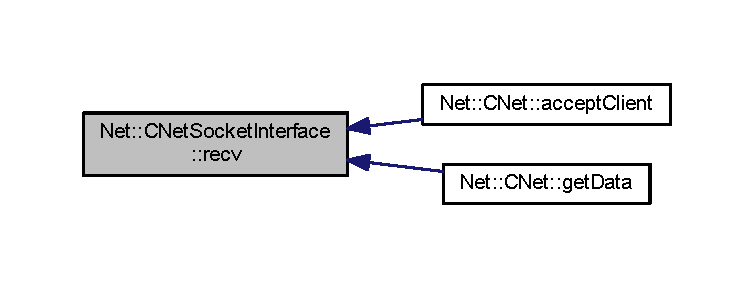
\includegraphics[width=350pt]{class_net_1_1_c_net_socket_interface_a66531da7c243f12948bd79293d6299e2_icgraph}
\end{center}
\end{figure}
\mbox{\Hypertarget{class_net_1_1_c_net_socket_interface_ad6a594a3ebe2fd855399aabfcbe0f95e}\label{class_net_1_1_c_net_socket_interface_ad6a594a3ebe2fd855399aabfcbe0f95e}} 
\index{Net\+::\+C\+Net\+Socket\+Interface@{Net\+::\+C\+Net\+Socket\+Interface}!send@{send}}
\index{send@{send}!Net\+::\+C\+Net\+Socket\+Interface@{Net\+::\+C\+Net\+Socket\+Interface}}
\subsubsection{\texorpdfstring{send()}{send()}}
{\footnotesize\ttfamily int Net\+::\+C\+Net\+Socket\+Interface\+::send (\begin{DoxyParamCaption}\item[{const int}]{socket,  }\item[{const char $\ast$}]{data,  }\item[{const int}]{data\+Size }\end{DoxyParamCaption})\hspace{0.3cm}{\ttfamily [static]}}



Sending data. 


\begin{DoxyParams}{Parameters}
{\em socket} & \\
\hline
{\em data} & \\
\hline
{\em data\+Size} & \\
\hline
\end{DoxyParams}
\begin{DoxyReturn}{Returns}
int The size of the sent data. -\/1 if an error occurred. 
\end{DoxyReturn}
Here is the caller graph for this function\+:
\nopagebreak
\begin{figure}[H]
\begin{center}
\leavevmode
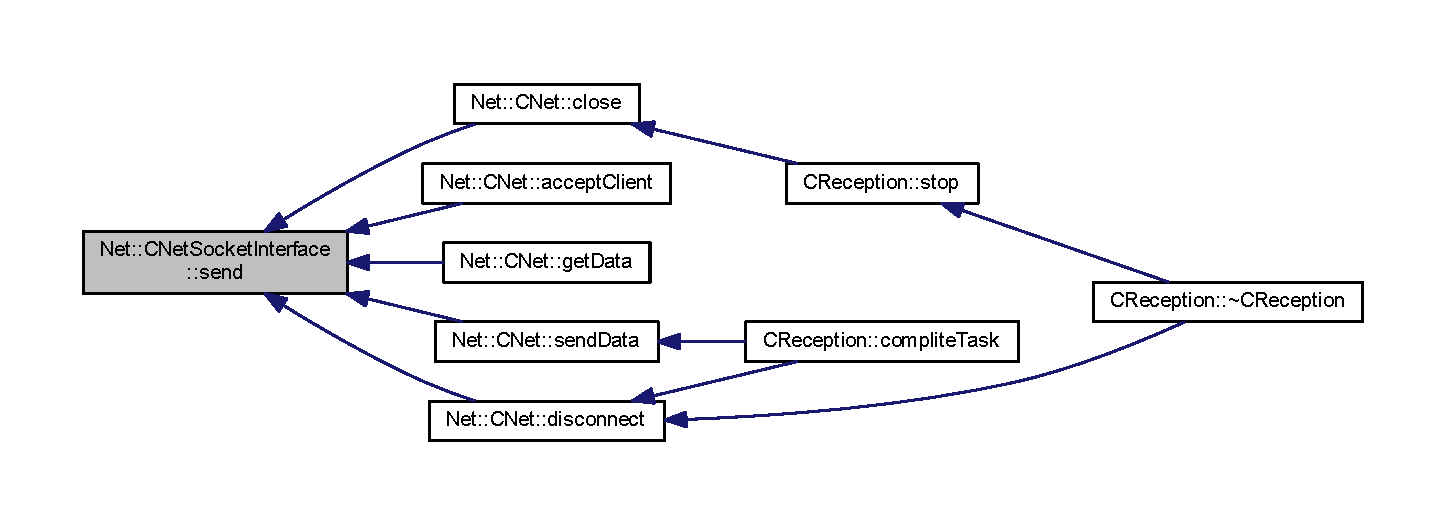
\includegraphics[width=350pt]{class_net_1_1_c_net_socket_interface_ad6a594a3ebe2fd855399aabfcbe0f95e_icgraph}
\end{center}
\end{figure}


The documentation for this class was generated from the following files\+:\begin{DoxyCompactItemize}
\item 
server/\+C\+Net/C\+Net\+Socket\+Interface.\+hpp\item 
server/\+C\+Net/C\+Net\+Socket\+Interface\+Linux.\+cpp\item 
server/\+C\+Net/C\+Net\+Socket\+Interface\+Windows.\+cpp\end{DoxyCompactItemize}

\hypertarget{class_c_reception}{}\section{C\+Reception Class Reference}
\label{class_c_reception}\index{C\+Reception@{C\+Reception}}


A class for asynchronous task acceptance from clients.  




{\ttfamily \#include $<$C\+Reception.\+hpp$>$}



Collaboration diagram for C\+Reception\+:
\nopagebreak
\begin{figure}[H]
\begin{center}
\leavevmode
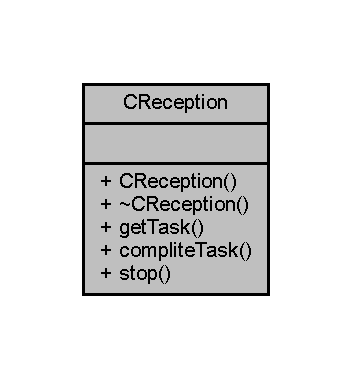
\includegraphics[width=169pt]{class_c_reception__coll__graph}
\end{center}
\end{figure}
\subsection*{Public Member Functions}
\begin{DoxyCompactItemize}
\item 
\mbox{\hyperlink{class_c_reception_a978822b58f7e3ec745869c9649c6dd14}{C\+Reception}} (const int max\+Con, const char $\ast$ip, const int port)
\begin{DoxyCompactList}\small\item\em Constructor. \end{DoxyCompactList}\item 
\mbox{\Hypertarget{class_c_reception_a6332fe59732e3eb5c2c6f5efecaaa2c5}\label{class_c_reception_a6332fe59732e3eb5c2c6f5efecaaa2c5}} 
\mbox{\hyperlink{class_c_reception_a6332fe59732e3eb5c2c6f5efecaaa2c5}{$\sim$\+C\+Reception}} ()
\begin{DoxyCompactList}\small\item\em Destructor. \end{DoxyCompactList}\item 
\mbox{\hyperlink{struct_s_task}{S\+Task}} \mbox{\hyperlink{class_c_reception_a842ffb5e64b4e65ff9faa087ffcd31fe}{get\+Task}} ()
\begin{DoxyCompactList}\small\item\em Getting the task. \end{DoxyCompactList}\item 
void \mbox{\hyperlink{class_c_reception_a286512c534ff02e51e8217241dd89727}{complite\+Task}} (\mbox{\hyperlink{struct_s_task}{S\+Task}} \&task)
\begin{DoxyCompactList}\small\item\em Sending the completed task. \end{DoxyCompactList}\item 
\mbox{\Hypertarget{class_c_reception_ae29e31358d6a1e7f410f3f07d93793ba}\label{class_c_reception_ae29e31358d6a1e7f410f3f07d93793ba}} 
void \mbox{\hyperlink{class_c_reception_ae29e31358d6a1e7f410f3f07d93793ba}{stop}} ()
\begin{DoxyCompactList}\small\item\em The function of stopping the work of receiving clients. \end{DoxyCompactList}\end{DoxyCompactItemize}


\subsection{Detailed Description}
A class for asynchronous task acceptance from clients. 

\subsection{Constructor \& Destructor Documentation}
\mbox{\Hypertarget{class_c_reception_a978822b58f7e3ec745869c9649c6dd14}\label{class_c_reception_a978822b58f7e3ec745869c9649c6dd14}} 
\index{C\+Reception@{C\+Reception}!C\+Reception@{C\+Reception}}
\index{C\+Reception@{C\+Reception}!C\+Reception@{C\+Reception}}
\subsubsection{\texorpdfstring{C\+Reception()}{CReception()}}
{\footnotesize\ttfamily C\+Reception\+::\+C\+Reception (\begin{DoxyParamCaption}\item[{const int}]{max\+Con,  }\item[{const char $\ast$}]{ip,  }\item[{const int}]{port }\end{DoxyParamCaption})}



Constructor. 


\begin{DoxyParams}{Parameters}
{\em max\+Con} & Maximum number of connections. \\
\hline
{\em ip} & I\+Pv4. \\
\hline
{\em port} & Port number. \\
\hline
\end{DoxyParams}


\subsection{Member Function Documentation}
\mbox{\Hypertarget{class_c_reception_a286512c534ff02e51e8217241dd89727}\label{class_c_reception_a286512c534ff02e51e8217241dd89727}} 
\index{C\+Reception@{C\+Reception}!complite\+Task@{complite\+Task}}
\index{complite\+Task@{complite\+Task}!C\+Reception@{C\+Reception}}
\subsubsection{\texorpdfstring{complite\+Task()}{compliteTask()}}
{\footnotesize\ttfamily void C\+Reception\+::complite\+Task (\begin{DoxyParamCaption}\item[{\mbox{\hyperlink{struct_s_task}{S\+Task}} \&}]{task }\end{DoxyParamCaption})}



Sending the completed task. 


\begin{DoxyParams}{Parameters}
{\em task} & Сompleted task. \\
\hline
\end{DoxyParams}
Here is the call graph for this function\+:
\nopagebreak
\begin{figure}[H]
\begin{center}
\leavevmode
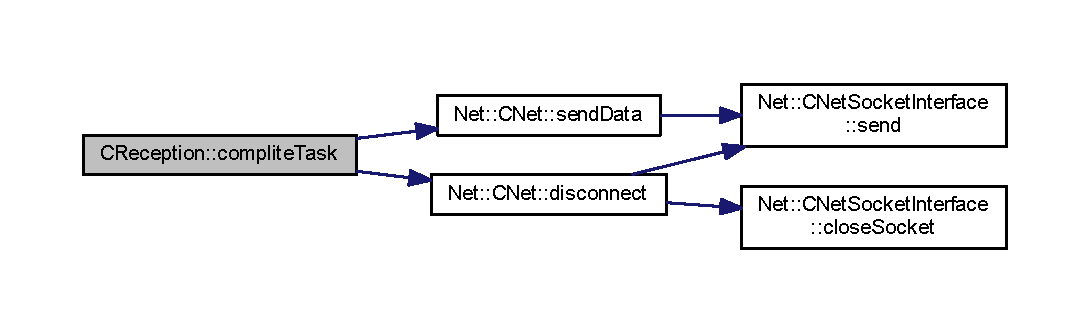
\includegraphics[width=350pt]{class_c_reception_a286512c534ff02e51e8217241dd89727_cgraph}
\end{center}
\end{figure}
\mbox{\Hypertarget{class_c_reception_a842ffb5e64b4e65ff9faa087ffcd31fe}\label{class_c_reception_a842ffb5e64b4e65ff9faa087ffcd31fe}} 
\index{C\+Reception@{C\+Reception}!get\+Task@{get\+Task}}
\index{get\+Task@{get\+Task}!C\+Reception@{C\+Reception}}
\subsubsection{\texorpdfstring{get\+Task()}{getTask()}}
{\footnotesize\ttfamily \mbox{\hyperlink{struct_s_task}{S\+Task}} C\+Reception\+::get\+Task (\begin{DoxyParamCaption}{ }\end{DoxyParamCaption})}



Getting the task. 

\begin{DoxyReturn}{Returns}
\mbox{\hyperlink{struct_s_task}{S\+Task}} 
\end{DoxyReturn}


The documentation for this class was generated from the following files\+:\begin{DoxyCompactItemize}
\item 
server/C\+Reception.\+hpp\item 
server/C\+Reception.\+cpp\end{DoxyCompactItemize}

\hypertarget{class_c_server}{}\section{C\+Server Class Reference}
\label{class_c_server}\index{C\+Server@{C\+Server}}


The class is a stream. which performs the work of the server.  




{\ttfamily \#include $<$C\+Server.\+hpp$>$}



Collaboration diagram for C\+Server\+:
\nopagebreak
\begin{figure}[H]
\begin{center}
\leavevmode
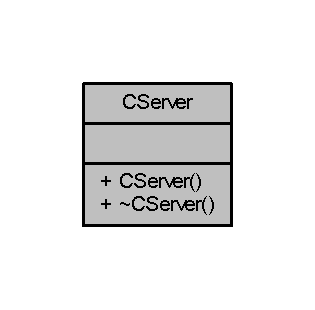
\includegraphics[width=151pt]{class_c_server__coll__graph}
\end{center}
\end{figure}


\subsection{Detailed Description}
The class is a stream. which performs the work of the server. 

The documentation for this class was generated from the following files\+:\begin{DoxyCompactItemize}
\item 
server/C\+Server.\+hpp\item 
server/C\+Server.\+cpp\end{DoxyCompactItemize}

\hypertarget{class_c_settings_manager}{}\section{C\+Settings\+Manager Class Reference}
\label{class_c_settings_manager}\index{C\+Settings\+Manager@{C\+Settings\+Manager}}


{\ttfamily \#include $<$C\+Settings\+Manager.\+hpp$>$}



Collaboration diagram for C\+Settings\+Manager\+:
\nopagebreak
\begin{figure}[H]
\begin{center}
\leavevmode
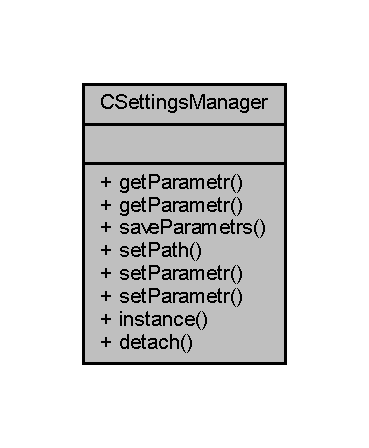
\includegraphics[width=177pt]{class_c_settings_manager__coll__graph}
\end{center}
\end{figure}
\subsection*{Public Member Functions}
\begin{DoxyCompactItemize}
\item 
bool \mbox{\hyperlink{class_c_settings_manager_ad0796e880134f641f6517d9a5433a877}{get\+Parametr}} (const std\+::string \&category, const std\+::string \&data\+Name, std\+::string \&parametr)
\item 
bool \mbox{\hyperlink{class_c_settings_manager_a6f45d4eaf3c79250f41bbac303b7c485}{get\+Parametr}} (const std\+::string \&category, const std\+::string \&data\+Name, int \&parametr)
\item 
bool \mbox{\hyperlink{class_c_settings_manager_a874956b5cb03b94bbb85ae0a5b25733f}{save\+Parametrs}} ()
\item 
void \mbox{\hyperlink{class_c_settings_manager_af67d1a3761332974fa0133e9d9819035}{set\+Path}} (const std\+::string \&path)
\item 
bool \mbox{\hyperlink{class_c_settings_manager_aa9efd965120731844f8ff2c2c994e638}{set\+Parametr}} (const std\+::string \&category, const std\+::string \&data\+Name, const std\+::string \&parametr)
\item 
bool \mbox{\hyperlink{class_c_settings_manager_a220fab46b436b6ded0ef311515a66899}{set\+Parametr}} (const std\+::string \&category, const std\+::string \&data\+Name, const int \&parametr)
\end{DoxyCompactItemize}
\subsection*{Static Public Member Functions}
\begin{DoxyCompactItemize}
\item 
static \mbox{\hyperlink{class_c_settings_manager}{C\+Settings\+Manager}} \& \mbox{\hyperlink{class_c_settings_manager_a40c0ffaf515eb306a9f83e3d631bcd21}{instance}} ()
\item 
static void \mbox{\hyperlink{class_c_settings_manager_a64524171654c8a7076af9ac9ac780bfc}{detach}} ()
\end{DoxyCompactItemize}


\subsection{Detailed Description}
The class that manages the settings files.

Static class. When the program is terminated, it is necessary to call method \begin{DoxySeeAlso}{See also}
\mbox{\hyperlink{class_c_settings_manager_a64524171654c8a7076af9ac9ac780bfc}{C\+Settings\+Manager\+::detach}}. You also need to call the 

\mbox{\hyperlink{class_c_settings_manager_a874956b5cb03b94bbb85ae0a5b25733f}{C\+Settings\+Manager\+::save\+Parametrs}} method to write the settings to files. 
\end{DoxySeeAlso}


\subsection{Member Function Documentation}
\mbox{\Hypertarget{class_c_settings_manager_a64524171654c8a7076af9ac9ac780bfc}\label{class_c_settings_manager_a64524171654c8a7076af9ac9ac780bfc}} 
\index{C\+Settings\+Manager@{C\+Settings\+Manager}!detach@{detach}}
\index{detach@{detach}!C\+Settings\+Manager@{C\+Settings\+Manager}}
\subsubsection{\texorpdfstring{detach()}{detach()}}
{\footnotesize\ttfamily void C\+Settings\+Manager\+::detach (\begin{DoxyParamCaption}{ }\end{DoxyParamCaption})\hspace{0.3cm}{\ttfamily [static]}}

Release of resources.

Not a thread-\/safe function. \mbox{\Hypertarget{class_c_settings_manager_ad0796e880134f641f6517d9a5433a877}\label{class_c_settings_manager_ad0796e880134f641f6517d9a5433a877}} 
\index{C\+Settings\+Manager@{C\+Settings\+Manager}!get\+Parametr@{get\+Parametr}}
\index{get\+Parametr@{get\+Parametr}!C\+Settings\+Manager@{C\+Settings\+Manager}}
\subsubsection{\texorpdfstring{get\+Parametr()}{getParametr()}\hspace{0.1cm}{\footnotesize\ttfamily [1/2]}}
{\footnotesize\ttfamily bool C\+Settings\+Manager\+::get\+Parametr (\begin{DoxyParamCaption}\item[{const std\+::string \&}]{category,  }\item[{const std\+::string \&}]{data\+Name,  }\item[{std\+::string \&}]{parametr }\end{DoxyParamCaption})}

Function of obtaining parameters.

Looks for among the loaded categories and looks for the required parameter. If the category is not found, it tries to load the \char`\"{}category\char`\"{}.conf file. Thread safe function.


\begin{DoxyParams}[1]{Parameters}
\mbox{\tt in}  & {\em category} & The name of the category (File name) that contains the parameter. \\
\hline
\mbox{\tt in}  & {\em data\+Name} & Parametr name. \\
\hline
\mbox{\tt out}  & {\em parametr} & Requested data.\\
\hline
\end{DoxyParams}
\begin{DoxyReturn}{Returns}
true Returns true if the parameter was found successfully, otherwise false. 
\end{DoxyReturn}
\mbox{\Hypertarget{class_c_settings_manager_a6f45d4eaf3c79250f41bbac303b7c485}\label{class_c_settings_manager_a6f45d4eaf3c79250f41bbac303b7c485}} 
\index{C\+Settings\+Manager@{C\+Settings\+Manager}!get\+Parametr@{get\+Parametr}}
\index{get\+Parametr@{get\+Parametr}!C\+Settings\+Manager@{C\+Settings\+Manager}}
\subsubsection{\texorpdfstring{get\+Parametr()}{getParametr()}\hspace{0.1cm}{\footnotesize\ttfamily [2/2]}}
{\footnotesize\ttfamily bool C\+Settings\+Manager\+::get\+Parametr (\begin{DoxyParamCaption}\item[{const std\+::string \&}]{category,  }\item[{const std\+::string \&}]{data\+Name,  }\item[{int \&}]{parametr }\end{DoxyParamCaption})}

Get integer parametr. \begin{DoxySeeAlso}{See also}
\mbox{\hyperlink{class_c_settings_manager_ad0796e880134f641f6517d9a5433a877}{C\+Settings\+Manager\+::get\+Parametr}} 
\end{DoxySeeAlso}
\mbox{\Hypertarget{class_c_settings_manager_a40c0ffaf515eb306a9f83e3d631bcd21}\label{class_c_settings_manager_a40c0ffaf515eb306a9f83e3d631bcd21}} 
\index{C\+Settings\+Manager@{C\+Settings\+Manager}!instance@{instance}}
\index{instance@{instance}!C\+Settings\+Manager@{C\+Settings\+Manager}}
\subsubsection{\texorpdfstring{instance()}{instance()}}
{\footnotesize\ttfamily \mbox{\hyperlink{class_c_settings_manager}{C\+Settings\+Manager}} \& C\+Settings\+Manager\+::instance (\begin{DoxyParamCaption}{ }\end{DoxyParamCaption})\hspace{0.3cm}{\ttfamily [static]}}

Get instance.

Not a thread-\/safe function. \mbox{\Hypertarget{class_c_settings_manager_a874956b5cb03b94bbb85ae0a5b25733f}\label{class_c_settings_manager_a874956b5cb03b94bbb85ae0a5b25733f}} 
\index{C\+Settings\+Manager@{C\+Settings\+Manager}!save\+Parametrs@{save\+Parametrs}}
\index{save\+Parametrs@{save\+Parametrs}!C\+Settings\+Manager@{C\+Settings\+Manager}}
\subsubsection{\texorpdfstring{save\+Parametrs()}{saveParametrs()}}
{\footnotesize\ttfamily bool C\+Settings\+Manager\+::save\+Parametrs (\begin{DoxyParamCaption}{ }\end{DoxyParamCaption})}

Writes parameters to files.

Thread safe function.

\begin{DoxyReturn}{Returns}
True if success write. 
\end{DoxyReturn}
\mbox{\Hypertarget{class_c_settings_manager_aa9efd965120731844f8ff2c2c994e638}\label{class_c_settings_manager_aa9efd965120731844f8ff2c2c994e638}} 
\index{C\+Settings\+Manager@{C\+Settings\+Manager}!set\+Parametr@{set\+Parametr}}
\index{set\+Parametr@{set\+Parametr}!C\+Settings\+Manager@{C\+Settings\+Manager}}
\subsubsection{\texorpdfstring{set\+Parametr()}{setParametr()}\hspace{0.1cm}{\footnotesize\ttfamily [1/2]}}
{\footnotesize\ttfamily bool C\+Settings\+Manager\+::set\+Parametr (\begin{DoxyParamCaption}\item[{const std\+::string \&}]{category,  }\item[{const std\+::string \&}]{data\+Name,  }\item[{const std\+::string \&}]{parametr }\end{DoxyParamCaption})}

Parameter entry function.

Looks for among the loaded categories and looks for the required parameter. If the category is not found, it tries to load the \char`\"{}category\char`\"{}.conf file. Thread safe function.


\begin{DoxyParams}[1]{Parameters}
\mbox{\tt in}  & {\em category} & The name of the category (File name) that contains the parameter. \\
\hline
\mbox{\tt in}  & {\em data\+Name} & Parametr name. \\
\hline
\mbox{\tt in}  & {\em parametr} & New data.\\
\hline
\end{DoxyParams}
\begin{DoxyReturn}{Returns}
true Returns true if the parameter was set successfully, otherwise false. 
\end{DoxyReturn}
\mbox{\Hypertarget{class_c_settings_manager_a220fab46b436b6ded0ef311515a66899}\label{class_c_settings_manager_a220fab46b436b6ded0ef311515a66899}} 
\index{C\+Settings\+Manager@{C\+Settings\+Manager}!set\+Parametr@{set\+Parametr}}
\index{set\+Parametr@{set\+Parametr}!C\+Settings\+Manager@{C\+Settings\+Manager}}
\subsubsection{\texorpdfstring{set\+Parametr()}{setParametr()}\hspace{0.1cm}{\footnotesize\ttfamily [2/2]}}
{\footnotesize\ttfamily bool C\+Settings\+Manager\+::set\+Parametr (\begin{DoxyParamCaption}\item[{const std\+::string \&}]{category,  }\item[{const std\+::string \&}]{data\+Name,  }\item[{const int \&}]{parametr }\end{DoxyParamCaption})}

Parameter entry function.

Looks for among the loaded categories and looks for the required parameter. If the category is not found, it tries to load the $<$category$>$.conf file. Thread safe function.


\begin{DoxyParams}[1]{Parameters}
\mbox{\tt in}  & {\em category} & The name of the category (File name) that contains the parameter. \\
\hline
\mbox{\tt in}  & {\em data\+Name} & Parametr name. \\
\hline
\mbox{\tt in}  & {\em parametr} & New data.\\
\hline
\end{DoxyParams}
\begin{DoxyReturn}{Returns}
true Returns true if the parameter was set successfully, otherwise false. 
\end{DoxyReturn}
\mbox{\Hypertarget{class_c_settings_manager_af67d1a3761332974fa0133e9d9819035}\label{class_c_settings_manager_af67d1a3761332974fa0133e9d9819035}} 
\index{C\+Settings\+Manager@{C\+Settings\+Manager}!set\+Path@{set\+Path}}
\index{set\+Path@{set\+Path}!C\+Settings\+Manager@{C\+Settings\+Manager}}
\subsubsection{\texorpdfstring{set\+Path()}{setPath()}}
{\footnotesize\ttfamily void C\+Settings\+Manager\+::set\+Path (\begin{DoxyParamCaption}\item[{const std\+::string \&}]{path }\end{DoxyParamCaption})}

Set path where stored $\ast$.conf files.

Thread safe function.


\begin{DoxyParams}[1]{Parameters}
\mbox{\tt in}  & {\em path} & Path to dirictory. \\
\hline
\end{DoxyParams}


The documentation for this class was generated from the following files\+:\begin{DoxyCompactItemize}
\item 
settings\+Manager/include/C\+Settings\+Manager.\+hpp\item 
settings\+Manager/src/C\+Settings\+Manager.\+cpp\end{DoxyCompactItemize}

\hypertarget{class_c_water_compute}{}\section{C\+Water\+Compute Class Reference}
\label{class_c_water_compute}\index{C\+Water\+Compute@{C\+Water\+Compute}}


{\ttfamily \#include $<$C\+Water\+Compute.\+hpp$>$}



Inheritance diagram for C\+Water\+Compute\+:
\nopagebreak
\begin{figure}[H]
\begin{center}
\leavevmode
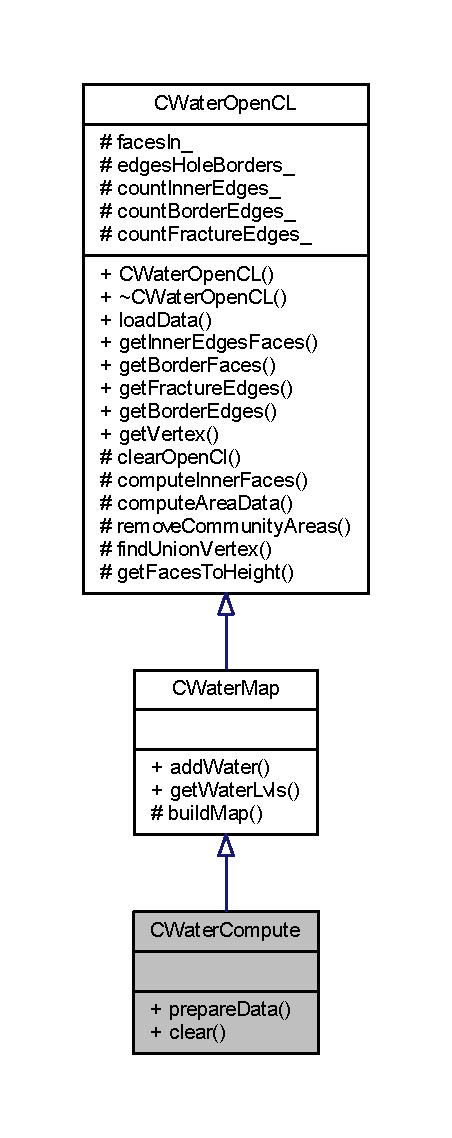
\includegraphics[width=217pt]{class_c_water_compute__inherit__graph}
\end{center}
\end{figure}


Collaboration diagram for C\+Water\+Compute\+:
\nopagebreak
\begin{figure}[H]
\begin{center}
\leavevmode
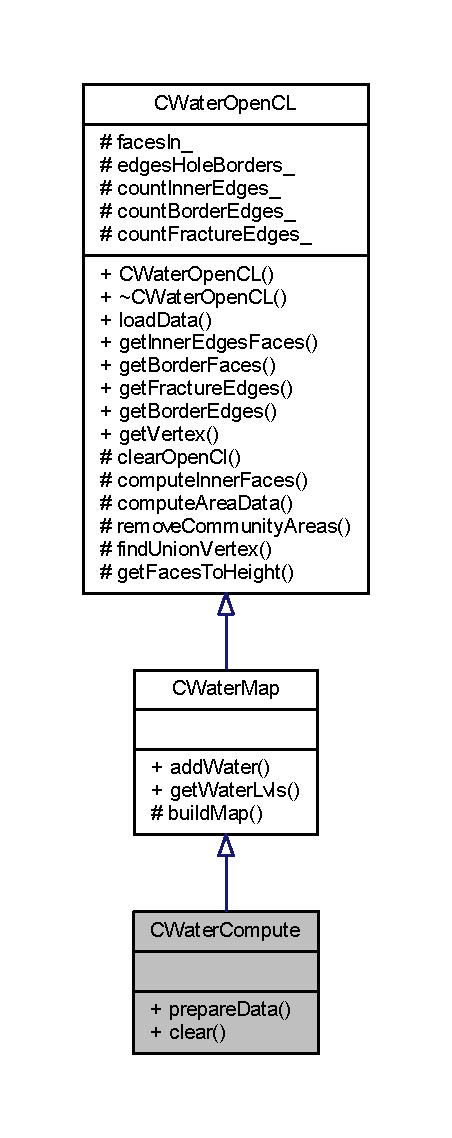
\includegraphics[width=217pt]{class_c_water_compute__coll__graph}
\end{center}
\end{figure}
\subsection*{Public Member Functions}
\begin{DoxyCompactItemize}
\item 
int \mbox{\hyperlink{class_c_water_compute_a5486835df389547dea8403401738c071}{prepare\+Data}} ()
\item 
void \mbox{\hyperlink{class_c_water_compute_a6afba6407dd75a22e2beeac9472fdf6c}{clear}} ()
\end{DoxyCompactItemize}
\subsection*{Additional Inherited Members}


\subsection{Detailed Description}
Class of basic calculations. 

\subsection{Member Function Documentation}
\mbox{\Hypertarget{class_c_water_compute_a6afba6407dd75a22e2beeac9472fdf6c}\label{class_c_water_compute_a6afba6407dd75a22e2beeac9472fdf6c}} 
\index{C\+Water\+Compute@{C\+Water\+Compute}!clear@{clear}}
\index{clear@{clear}!C\+Water\+Compute@{C\+Water\+Compute}}
\subsubsection{\texorpdfstring{clear()}{clear()}}
{\footnotesize\ttfamily void C\+Water\+Compute\+::clear (\begin{DoxyParamCaption}{ }\end{DoxyParamCaption})}

Cleaning of internal data. Here is the call graph for this function\+:
\nopagebreak
\begin{figure}[H]
\begin{center}
\leavevmode
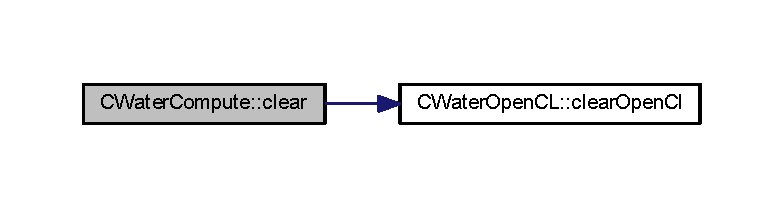
\includegraphics[width=350pt]{class_c_water_compute_a6afba6407dd75a22e2beeac9472fdf6c_cgraph}
\end{center}
\end{figure}
\mbox{\Hypertarget{class_c_water_compute_a5486835df389547dea8403401738c071}\label{class_c_water_compute_a5486835df389547dea8403401738c071}} 
\index{C\+Water\+Compute@{C\+Water\+Compute}!prepare\+Data@{prepare\+Data}}
\index{prepare\+Data@{prepare\+Data}!C\+Water\+Compute@{C\+Water\+Compute}}
\subsubsection{\texorpdfstring{prepare\+Data()}{prepareData()}}
{\footnotesize\ttfamily int C\+Water\+Compute\+::prepare\+Data (\begin{DoxyParamCaption}{ }\end{DoxyParamCaption})}

Prepare data to calculates water levels. 
\begin{DoxyParams}{Parameters}
{\em vertex} & Buffer for output data about vertices. \\
\hline
{\em Buffer} & for output data about polygons. \\
\hline
\end{DoxyParams}
\begin{DoxyReturn}{Returns}
0 if sucsses, else Open\+Cl error code. 
\end{DoxyReturn}


The documentation for this class was generated from the following files\+:\begin{DoxyCompactItemize}
\item 
water\+Compute/include/C\+Water\+Compute.\+hpp\item 
water\+Compute/src/C\+Water\+Compute.\+cpp\end{DoxyCompactItemize}

\hypertarget{class_c_water_map}{}\section{C\+Water\+Map Class Reference}
\label{class_c_water_map}\index{C\+Water\+Map@{C\+Water\+Map}}


{\ttfamily \#include $<$C\+Water\+Map.\+hpp$>$}



Inheritance diagram for C\+Water\+Map\+:
\nopagebreak
\begin{figure}[H]
\begin{center}
\leavevmode
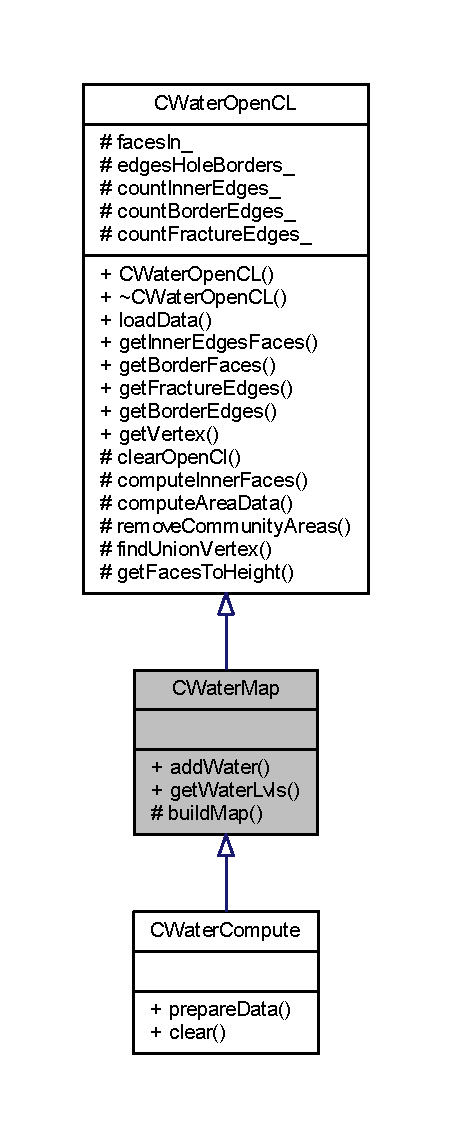
\includegraphics[width=217pt]{class_c_water_map__inherit__graph}
\end{center}
\end{figure}


Collaboration diagram for C\+Water\+Map\+:
\nopagebreak
\begin{figure}[H]
\begin{center}
\leavevmode
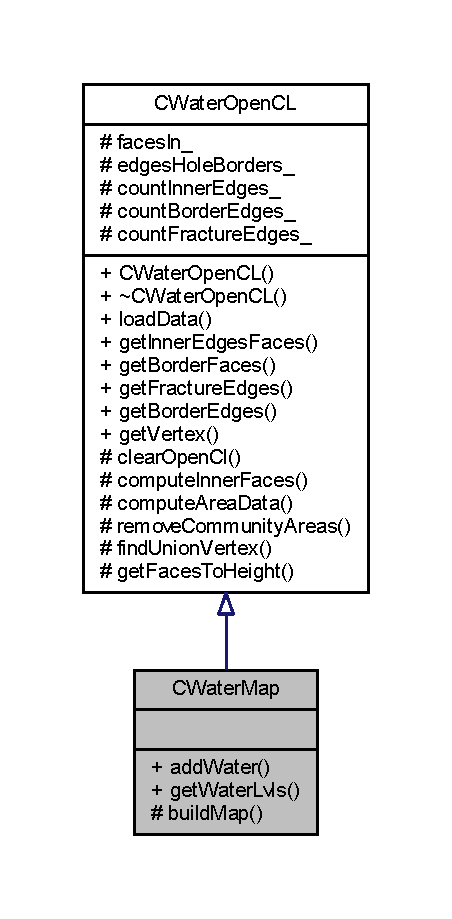
\includegraphics[width=217pt]{class_c_water_map__coll__graph}
\end{center}
\end{figure}
\subsection*{Public Member Functions}
\begin{DoxyCompactItemize}
\item 
\mbox{\Hypertarget{class_c_water_map_a99ee0ad6fdbf8f07617d4f5b4c759bcd}\label{class_c_water_map_a99ee0ad6fdbf8f07617d4f5b4c759bcd}} 
void {\bfseries add\+Water} (const float size)
\item 
\mbox{\Hypertarget{class_c_water_map_aca1fa16390fe2a39e4d576045f3404e9}\label{class_c_water_map_aca1fa16390fe2a39e4d576045f3404e9}} 
void {\bfseries get\+Water\+Lvls} (std\+::list$<$ std\+::vector$<$ float $>$$>$ \&vertex, std\+::list$<$ std\+::vector$<$ uint32\+\_\+t $>$$>$ \&faces)
\end{DoxyCompactItemize}
\subsection*{Protected Member Functions}
\begin{DoxyCompactItemize}
\item 
\mbox{\Hypertarget{class_c_water_map_a3dcda9c5dd50d45f317e526c6949f8db}\label{class_c_water_map_a3dcda9c5dd50d45f317e526c6949f8db}} 
int {\bfseries build\+Map} (const std\+::list$<$ std\+::vector$<$ uint32\+\_\+t $>$$>$ \&borders, const std\+::list$<$ std\+::vector$<$ uint32\+\_\+t $>$$>$ \&areas)
\end{DoxyCompactItemize}
\subsection*{Additional Inherited Members}


\subsection{Detailed Description}
Class of basic calculations. 

The documentation for this class was generated from the following files\+:\begin{DoxyCompactItemize}
\item 
water\+Compute/include/C\+Water\+Map.\+hpp\item 
water\+Compute/src/C\+Water\+Map.\+cpp\end{DoxyCompactItemize}

\hypertarget{class_c_water_open_c_l}{}\section{C\+Water\+Open\+CL Class Reference}
\label{class_c_water_open_c_l}\index{C\+Water\+Open\+CL@{C\+Water\+Open\+CL}}


{\ttfamily \#include $<$C\+Water\+Open\+C\+L.\+hpp$>$}



Inheritance diagram for C\+Water\+Open\+CL\+:
\nopagebreak
\begin{figure}[H]
\begin{center}
\leavevmode
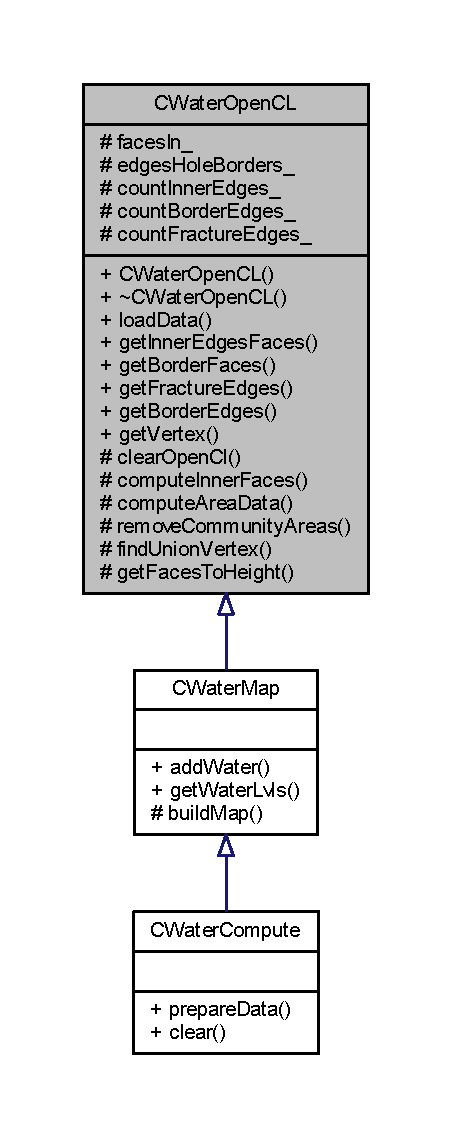
\includegraphics[width=217pt]{class_c_water_open_c_l__inherit__graph}
\end{center}
\end{figure}


Collaboration diagram for C\+Water\+Open\+CL\+:
\nopagebreak
\begin{figure}[H]
\begin{center}
\leavevmode
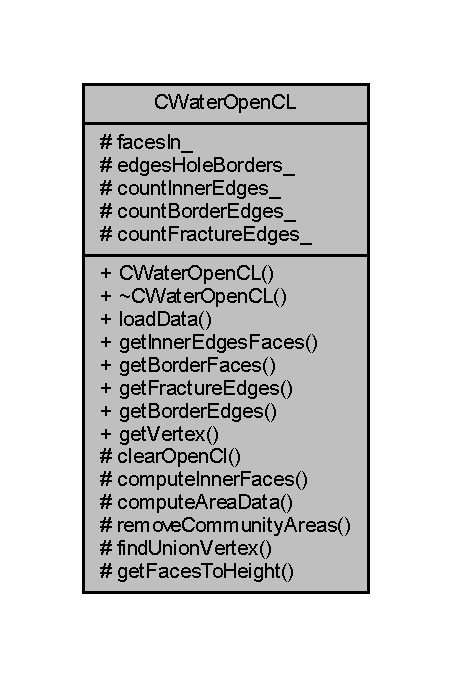
\includegraphics[width=217pt]{class_c_water_open_c_l__coll__graph}
\end{center}
\end{figure}
\subsection*{Public Member Functions}
\begin{DoxyCompactItemize}
\item 
\mbox{\Hypertarget{class_c_water_open_c_l_a40ad7bc6720195721f3129aa8c2739d4}\label{class_c_water_open_c_l_a40ad7bc6720195721f3129aa8c2739d4}} 
int {\bfseries load\+Data} (const std\+::vector$<$ float $>$ \&vertex, const std\+::vector$<$ uint32\+\_\+t $>$ \&faces)
\item 
\mbox{\Hypertarget{class_c_water_open_c_l_a9e817028b963e53eba18e0c7591885e6}\label{class_c_water_open_c_l_a9e817028b963e53eba18e0c7591885e6}} 
int {\bfseries get\+Inner\+Edges\+Faces} (std\+::vector$<$ uint32\+\_\+t $>$ \&faces) const
\item 
\mbox{\Hypertarget{class_c_water_open_c_l_ab2e33f7535616c17a9e93fd92a0664b2}\label{class_c_water_open_c_l_ab2e33f7535616c17a9e93fd92a0664b2}} 
int {\bfseries get\+Border\+Faces} (std\+::vector$<$ uint32\+\_\+t $>$ \&faces) const
\item 
\mbox{\Hypertarget{class_c_water_open_c_l_a9b09f2f3bd783f601ee34981bc26c112}\label{class_c_water_open_c_l_a9b09f2f3bd783f601ee34981bc26c112}} 
int {\bfseries get\+Fracture\+Edges} (std\+::vector$<$ uint32\+\_\+t $>$ \&edges) const
\item 
\mbox{\Hypertarget{class_c_water_open_c_l_ab935c58d2c24c2739988d980cec389b8}\label{class_c_water_open_c_l_ab935c58d2c24c2739988d980cec389b8}} 
int {\bfseries get\+Border\+Edges} (std\+::vector$<$ uint32\+\_\+t $>$ \&edges) const
\item 
\mbox{\Hypertarget{class_c_water_open_c_l_ac99522af5b8a9653beb5cdafc456d454}\label{class_c_water_open_c_l_ac99522af5b8a9653beb5cdafc456d454}} 
int {\bfseries get\+Vertex} (std\+::vector$<$ float $>$ \&result) const
\end{DoxyCompactItemize}
\subsection*{Protected Member Functions}
\begin{DoxyCompactItemize}
\item 
void \mbox{\hyperlink{class_c_water_open_c_l_a213bd842a23c3a1d50e90b60d9395143}{clear\+Open\+Cl}} ()
\item 
\mbox{\Hypertarget{class_c_water_open_c_l_af270a8ce81a691fd166ef1548a740d75}\label{class_c_water_open_c_l_af270a8ce81a691fd166ef1548a740d75}} 
int {\bfseries compute\+Inner\+Faces} (const std\+::list$<$ std\+::vector$<$ uint32\+\_\+t $>$$>$ \&borders, std\+::list$<$ std\+::vector$<$ uint32\+\_\+t $>$$>$ \&faces)
\item 
\mbox{\Hypertarget{class_c_water_open_c_l_a30713ebb73035f4b64dbf2a392b33d72}\label{class_c_water_open_c_l_a30713ebb73035f4b64dbf2a392b33d72}} 
int {\bfseries compute\+Area\+Data} (const std\+::list$<$ std\+::vector$<$ uint32\+\_\+t $>$$>$ \&areas, const std\+::vector$<$ float $>$ \&heights, std\+::vector$<$ float $>$ \&result\+Square, std\+::vector$<$ float $>$ \&result\+Val)
\item 
\mbox{\Hypertarget{class_c_water_open_c_l_a67e69f0d1a0b9139bde5c8ded6a9137e}\label{class_c_water_open_c_l_a67e69f0d1a0b9139bde5c8ded6a9137e}} 
int {\bfseries remove\+Community\+Areas} (std\+::list$<$ std\+::vector$<$ uint32\+\_\+t $>$$>$ \&areas, std\+::list$<$ std\+::vector$<$ uint32\+\_\+t $>$$>$ \&new\+Areas)
\item 
\mbox{\Hypertarget{class_c_water_open_c_l_aad6a697a2579f3679a7574aaa30bb7ef}\label{class_c_water_open_c_l_aad6a697a2579f3679a7574aaa30bb7ef}} 
int {\bfseries find\+Union\+Vertex} (const std\+::list$<$ std\+::vector$<$ uint32\+\_\+t $>$$>$ \&areas, std\+::list$<$ std\+::vector$<$ uint32\+\_\+t $>$$>$ \&union\+Vertex)
\item 
\mbox{\Hypertarget{class_c_water_open_c_l_a6500cbf0c77d5b262374d69763de09a0}\label{class_c_water_open_c_l_a6500cbf0c77d5b262374d69763de09a0}} 
int {\bfseries get\+Faces\+To\+Height} (const std\+::vector$<$ uint32\+\_\+t $>$ \&area, const float height, std\+::vector$<$ uint32\+\_\+t $>$ \&faces, std\+::vector$<$ float $>$ \&vertex)
\end{DoxyCompactItemize}
\subsection*{Protected Attributes}
\begin{DoxyCompactItemize}
\item 
\mbox{\Hypertarget{class_c_water_open_c_l_ac737018fb1ad601bdb27e916bcba2dc9}\label{class_c_water_open_c_l_ac737018fb1ad601bdb27e916bcba2dc9}} 
std\+::vector$<$ uint32\+\_\+t $>$ {\bfseries faces\+In\+\_\+}
\item 
\mbox{\Hypertarget{class_c_water_open_c_l_ac77a547983236889023df42587eb5576}\label{class_c_water_open_c_l_ac77a547983236889023df42587eb5576}} 
std\+::vector$<$ uint32\+\_\+t $>$ {\bfseries edges\+Hole\+Borders\+\_\+}
\item 
\mbox{\Hypertarget{class_c_water_open_c_l_ac8ddc30747be7685da174f20d33976f2}\label{class_c_water_open_c_l_ac8ddc30747be7685da174f20d33976f2}} 
uint32\+\_\+t {\bfseries count\+Inner\+Edges\+\_\+} = 0
\item 
\mbox{\Hypertarget{class_c_water_open_c_l_a762f011180770ef178b923bd3afebb98}\label{class_c_water_open_c_l_a762f011180770ef178b923bd3afebb98}} 
uint32\+\_\+t {\bfseries count\+Border\+Edges\+\_\+} = 0
\item 
\mbox{\Hypertarget{class_c_water_open_c_l_a70cf05f1d4d723bc90d671fcf9c6ed85}\label{class_c_water_open_c_l_a70cf05f1d4d723bc90d671fcf9c6ed85}} 
uint32\+\_\+t {\bfseries count\+Fracture\+Edges\+\_\+} = 0
\end{DoxyCompactItemize}


\subsection{Detailed Description}
A class that performs parallel processing of data. 

\subsection{Member Function Documentation}
\mbox{\Hypertarget{class_c_water_open_c_l_a213bd842a23c3a1d50e90b60d9395143}\label{class_c_water_open_c_l_a213bd842a23c3a1d50e90b60d9395143}} 
\index{C\+Water\+Open\+CL@{C\+Water\+Open\+CL}!clear\+Open\+Cl@{clear\+Open\+Cl}}
\index{clear\+Open\+Cl@{clear\+Open\+Cl}!C\+Water\+Open\+CL@{C\+Water\+Open\+CL}}
\subsubsection{\texorpdfstring{clear\+Open\+Cl()}{clearOpenCl()}}
{\footnotesize\ttfamily void C\+Water\+Open\+C\+L\+::clear\+Open\+Cl (\begin{DoxyParamCaption}{ }\end{DoxyParamCaption})\hspace{0.3cm}{\ttfamily [protected]}}

Cleaning of internal data. Here is the caller graph for this function\+:
\nopagebreak
\begin{figure}[H]
\begin{center}
\leavevmode
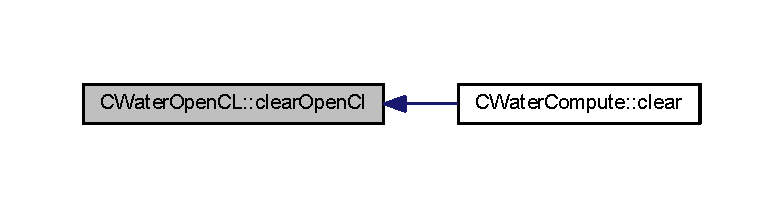
\includegraphics[width=350pt]{class_c_water_open_c_l_a213bd842a23c3a1d50e90b60d9395143_icgraph}
\end{center}
\end{figure}


The documentation for this class was generated from the following files\+:\begin{DoxyCompactItemize}
\item 
water\+Compute/include/C\+Water\+Open\+C\+L.\+hpp\item 
water\+Compute/src/C\+Water\+Open\+C\+L.\+cpp\end{DoxyCompactItemize}

\hypertarget{struct_net_1_1_s_message_head}{}\section{Net\+:\+:S\+Message\+Head Struct Reference}
\label{struct_net_1_1_s_message_head}\index{Net\+::\+S\+Message\+Head@{Net\+::\+S\+Message\+Head}}


Structure for storing the header of the decoded message.  




{\ttfamily \#include $<$C\+Net\+Handler.\+hpp$>$}



Collaboration diagram for Net\+:\+:S\+Message\+Head\+:
\nopagebreak
\begin{figure}[H]
\begin{center}
\leavevmode
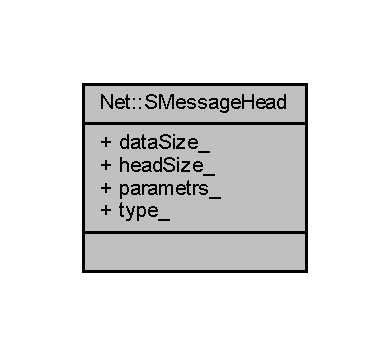
\includegraphics[width=187pt]{struct_net_1_1_s_message_head__coll__graph}
\end{center}
\end{figure}
\subsection*{Public Attributes}
\begin{DoxyCompactItemize}
\item 
\mbox{\Hypertarget{struct_net_1_1_s_message_head_a2e01a7a3434acdfc8e7342267fe26935}\label{struct_net_1_1_s_message_head_a2e01a7a3434acdfc8e7342267fe26935}} 
uint {\bfseries data\+Size\+\_\+} = 0
\item 
\mbox{\Hypertarget{struct_net_1_1_s_message_head_a93f8e120b7c67e935a42f5a130119983}\label{struct_net_1_1_s_message_head_a93f8e120b7c67e935a42f5a130119983}} 
uint {\bfseries head\+Size\+\_\+} = 0
\item 
\mbox{\Hypertarget{struct_net_1_1_s_message_head_a97d84a5454b38da45791c9fe4bcd2d6a}\label{struct_net_1_1_s_message_head_a97d84a5454b38da45791c9fe4bcd2d6a}} 
uint {\bfseries parametrs\+\_\+} = 0
\item 
\mbox{\Hypertarget{struct_net_1_1_s_message_head_a67e646e8fe21f7e21f91a3bf1010f248}\label{struct_net_1_1_s_message_head_a67e646e8fe21f7e21f91a3bf1010f248}} 
Message\+Type {\bfseries type\+\_\+} = E\+R\+R\+O\+R\+\_\+\+H\+E\+AD
\end{DoxyCompactItemize}


\subsection{Detailed Description}
Structure for storing the header of the decoded message. 

The documentation for this struct was generated from the following file\+:\begin{DoxyCompactItemize}
\item 
server/\+C\+Net/\+Handler/C\+Net\+Handler.\+hpp\end{DoxyCompactItemize}

\hypertarget{struct_s_task}{}\section{S\+Task Struct Reference}
\label{struct_s_task}\index{S\+Task@{S\+Task}}


Structure for storing task data.  




{\ttfamily \#include $<$C\+Reception.\+hpp$>$}



Collaboration diagram for S\+Task\+:
\nopagebreak
\begin{figure}[H]
\begin{center}
\leavevmode
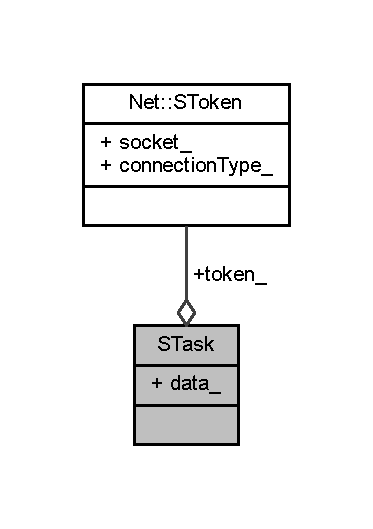
\includegraphics[width=179pt]{struct_s_task__coll__graph}
\end{center}
\end{figure}
\subsection*{Public Attributes}
\begin{DoxyCompactItemize}
\item 
\mbox{\Hypertarget{struct_s_task_ab0ca736167067e374c4e8860834d515b}\label{struct_s_task_ab0ca736167067e374c4e8860834d515b}} 
\mbox{\hyperlink{struct_net_1_1_s_token}{Net\+::\+S\+Token}} {\bfseries token\+\_\+}
\item 
\mbox{\Hypertarget{struct_s_task_a67c3bf7df4705a2b43270f32a90f824a}\label{struct_s_task_a67c3bf7df4705a2b43270f32a90f824a}} 
std\+::string {\bfseries data\+\_\+}
\end{DoxyCompactItemize}


\subsection{Detailed Description}
Structure for storing task data. 

The documentation for this struct was generated from the following file\+:\begin{DoxyCompactItemize}
\item 
server/C\+Reception.\+hpp\end{DoxyCompactItemize}

\hypertarget{struct_net_1_1_s_token}{}\section{Net\+:\+:S\+Token Struct Reference}
\label{struct_net_1_1_s_token}\index{Net\+::\+S\+Token@{Net\+::\+S\+Token}}


Structure for storing connection data.  




{\ttfamily \#include $<$C\+Net.\+hpp$>$}



Collaboration diagram for Net\+:\+:S\+Token\+:
\nopagebreak
\begin{figure}[H]
\begin{center}
\leavevmode
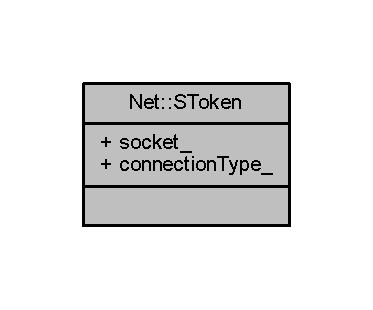
\includegraphics[width=179pt]{struct_net_1_1_s_token__coll__graph}
\end{center}
\end{figure}
\subsection*{Public Attributes}
\begin{DoxyCompactItemize}
\item 
\mbox{\Hypertarget{struct_net_1_1_s_token_aeecb14eb3dc790701699198cfa876916}\label{struct_net_1_1_s_token_aeecb14eb3dc790701699198cfa876916}} 
int {\bfseries socket\+\_\+} = -\/1
\item 
\mbox{\Hypertarget{struct_net_1_1_s_token_aa5a4724ed963dd892e3276ac0a52518e}\label{struct_net_1_1_s_token_aa5a4724ed963dd892e3276ac0a52518e}} 
uint {\bfseries connection\+Type\+\_\+}
\end{DoxyCompactItemize}


\subsection{Detailed Description}
Structure for storing connection data. 

The documentation for this struct was generated from the following file\+:\begin{DoxyCompactItemize}
\item 
server/\+C\+Net/C\+Net.\+hpp\end{DoxyCompactItemize}

\hypertarget{class_web_socket_handshake}{}\section{Web\+Socket\+Handshake Class Reference}
\label{class_web_socket_handshake}\index{Web\+Socket\+Handshake@{Web\+Socket\+Handshake}}


Collaboration diagram for Web\+Socket\+Handshake\+:
\nopagebreak
\begin{figure}[H]
\begin{center}
\leavevmode
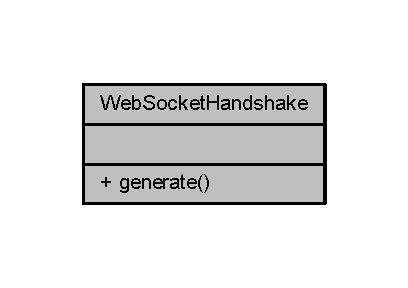
\includegraphics[width=196pt]{class_web_socket_handshake__coll__graph}
\end{center}
\end{figure}
\subsection*{Static Public Member Functions}
\begin{DoxyCompactItemize}
\item 
\mbox{\Hypertarget{class_web_socket_handshake_a7e9966dcd8135e90ccba3604d3739280}\label{class_web_socket_handshake_a7e9966dcd8135e90ccba3604d3739280}} 
static void {\bfseries generate} (const char input\mbox{[}24\mbox{]}, char output\mbox{[}28\mbox{]})
\end{DoxyCompactItemize}


The documentation for this class was generated from the following file\+:\begin{DoxyCompactItemize}
\item 
server/\+C\+Net/\+Handler/libwshandshake.\+hpp\end{DoxyCompactItemize}

%--- End generated contents ---

% Index
\backmatter
\newpage
\phantomsection
\clearemptydoublepage
\addcontentsline{toc}{chapter}{Index}
\printindex

\end{document}
